\documentclass[]{article}
\usepackage{lmodern}
\usepackage{amssymb,amsmath}
\usepackage{ifxetex,ifluatex}
\usepackage{fixltx2e} % provides \textsubscript
\ifnum 0\ifxetex 1\fi\ifluatex 1\fi=0 % if pdftex
  \usepackage[T1]{fontenc}
  \usepackage[utf8]{inputenc}
\else % if luatex or xelatex
  \ifxetex
    \usepackage{mathspec}
  \else
    \usepackage{fontspec}
  \fi
  \defaultfontfeatures{Ligatures=TeX,Scale=MatchLowercase}
\fi
% use upquote if available, for straight quotes in verbatim environments
\IfFileExists{upquote.sty}{\usepackage{upquote}}{}
% use microtype if available
\IfFileExists{microtype.sty}{%
\usepackage{microtype}
\UseMicrotypeSet[protrusion]{basicmath} % disable protrusion for tt fonts
}{}
\usepackage[margin=1in]{geometry}
\usepackage{hyperref}
\hypersetup{unicode=true,
            pdftitle={Clustering Algorithm for Unupervised Learning - Credit Card Client Anomaly Analysis},
            pdfauthor={Tyler Blakeley, Benjamin Kan, Mohammad Islam, Avijeet Singh},
            pdfborder={0 0 0},
            breaklinks=true}
\urlstyle{same}  % don't use monospace font for urls
\usepackage{color}
\usepackage{fancyvrb}
\newcommand{\VerbBar}{|}
\newcommand{\VERB}{\Verb[commandchars=\\\{\}]}
\DefineVerbatimEnvironment{Highlighting}{Verbatim}{commandchars=\\\{\}}
% Add ',fontsize=\small' for more characters per line
\usepackage{framed}
\definecolor{shadecolor}{RGB}{248,248,248}
\newenvironment{Shaded}{\begin{snugshade}}{\end{snugshade}}
\newcommand{\KeywordTok}[1]{\textcolor[rgb]{0.13,0.29,0.53}{\textbf{#1}}}
\newcommand{\DataTypeTok}[1]{\textcolor[rgb]{0.13,0.29,0.53}{#1}}
\newcommand{\DecValTok}[1]{\textcolor[rgb]{0.00,0.00,0.81}{#1}}
\newcommand{\BaseNTok}[1]{\textcolor[rgb]{0.00,0.00,0.81}{#1}}
\newcommand{\FloatTok}[1]{\textcolor[rgb]{0.00,0.00,0.81}{#1}}
\newcommand{\ConstantTok}[1]{\textcolor[rgb]{0.00,0.00,0.00}{#1}}
\newcommand{\CharTok}[1]{\textcolor[rgb]{0.31,0.60,0.02}{#1}}
\newcommand{\SpecialCharTok}[1]{\textcolor[rgb]{0.00,0.00,0.00}{#1}}
\newcommand{\StringTok}[1]{\textcolor[rgb]{0.31,0.60,0.02}{#1}}
\newcommand{\VerbatimStringTok}[1]{\textcolor[rgb]{0.31,0.60,0.02}{#1}}
\newcommand{\SpecialStringTok}[1]{\textcolor[rgb]{0.31,0.60,0.02}{#1}}
\newcommand{\ImportTok}[1]{#1}
\newcommand{\CommentTok}[1]{\textcolor[rgb]{0.56,0.35,0.01}{\textit{#1}}}
\newcommand{\DocumentationTok}[1]{\textcolor[rgb]{0.56,0.35,0.01}{\textbf{\textit{#1}}}}
\newcommand{\AnnotationTok}[1]{\textcolor[rgb]{0.56,0.35,0.01}{\textbf{\textit{#1}}}}
\newcommand{\CommentVarTok}[1]{\textcolor[rgb]{0.56,0.35,0.01}{\textbf{\textit{#1}}}}
\newcommand{\OtherTok}[1]{\textcolor[rgb]{0.56,0.35,0.01}{#1}}
\newcommand{\FunctionTok}[1]{\textcolor[rgb]{0.00,0.00,0.00}{#1}}
\newcommand{\VariableTok}[1]{\textcolor[rgb]{0.00,0.00,0.00}{#1}}
\newcommand{\ControlFlowTok}[1]{\textcolor[rgb]{0.13,0.29,0.53}{\textbf{#1}}}
\newcommand{\OperatorTok}[1]{\textcolor[rgb]{0.81,0.36,0.00}{\textbf{#1}}}
\newcommand{\BuiltInTok}[1]{#1}
\newcommand{\ExtensionTok}[1]{#1}
\newcommand{\PreprocessorTok}[1]{\textcolor[rgb]{0.56,0.35,0.01}{\textit{#1}}}
\newcommand{\AttributeTok}[1]{\textcolor[rgb]{0.77,0.63,0.00}{#1}}
\newcommand{\RegionMarkerTok}[1]{#1}
\newcommand{\InformationTok}[1]{\textcolor[rgb]{0.56,0.35,0.01}{\textbf{\textit{#1}}}}
\newcommand{\WarningTok}[1]{\textcolor[rgb]{0.56,0.35,0.01}{\textbf{\textit{#1}}}}
\newcommand{\AlertTok}[1]{\textcolor[rgb]{0.94,0.16,0.16}{#1}}
\newcommand{\ErrorTok}[1]{\textcolor[rgb]{0.64,0.00,0.00}{\textbf{#1}}}
\newcommand{\NormalTok}[1]{#1}
\usepackage{longtable,booktabs}
\usepackage{graphicx,grffile}
\makeatletter
\def\maxwidth{\ifdim\Gin@nat@width>\linewidth\linewidth\else\Gin@nat@width\fi}
\def\maxheight{\ifdim\Gin@nat@height>\textheight\textheight\else\Gin@nat@height\fi}
\makeatother
% Scale images if necessary, so that they will not overflow the page
% margins by default, and it is still possible to overwrite the defaults
% using explicit options in \includegraphics[width, height, ...]{}
\setkeys{Gin}{width=\maxwidth,height=\maxheight,keepaspectratio}
\IfFileExists{parskip.sty}{%
\usepackage{parskip}
}{% else
\setlength{\parindent}{0pt}
\setlength{\parskip}{6pt plus 2pt minus 1pt}
}
\setlength{\emergencystretch}{3em}  % prevent overfull lines
\providecommand{\tightlist}{%
  \setlength{\itemsep}{0pt}\setlength{\parskip}{0pt}}
\setcounter{secnumdepth}{0}
% Redefines (sub)paragraphs to behave more like sections
\ifx\paragraph\undefined\else
\let\oldparagraph\paragraph
\renewcommand{\paragraph}[1]{\oldparagraph{#1}\mbox{}}
\fi
\ifx\subparagraph\undefined\else
\let\oldsubparagraph\subparagraph
\renewcommand{\subparagraph}[1]{\oldsubparagraph{#1}\mbox{}}
\fi

%%% Use protect on footnotes to avoid problems with footnotes in titles
\let\rmarkdownfootnote\footnote%
\def\footnote{\protect\rmarkdownfootnote}

%%% Change title format to be more compact
\usepackage{titling}

% Create subtitle command for use in maketitle
\newcommand{\subtitle}[1]{
  \posttitle{
    \begin{center}\large#1\end{center}
    }
}

\setlength{\droptitle}{-2em}

  \title{Clustering Algorithm for Unupervised Learning - Credit Card Client
Anomaly Analysis}
    \pretitle{\vspace{\droptitle}\centering\huge}
  \posttitle{\par}
    \author{Tyler Blakeley, Benjamin Kan, Mohammad Islam, Avijeet Singh}
    \preauthor{\centering\large\emph}
  \postauthor{\par}
      \predate{\centering\large\emph}
  \postdate{\par}
    \date{October 29 2018}


\begin{document}
\maketitle

{
\setcounter{tocdepth}{2}
\tableofcontents
}
\section{Business Understanding}\label{business-understanding}

We work at the Retail Credit Risk Analytics department at the Bank of
Taiwan. Recently, there have been increasing credit card debt defaults
in our bank. Senior Management would like our department to develop a
machine learning algorithm to find anomalies in the data that we hope
will show early warning signs of default. This will allow the Retail
Credit Risk and Collections departments to act early by reducing these
cleints' credit card limits to minimize the losses. We would also like
to find out which demographics are in the anomaly group which would
indicate high susceptiblility of defaults. The Management instructed us
to use data from the third parties to build the algorithms as
proof-of-concepts before we use our own data. They would also like us to
build a user-friendly app to allow them to load in the dataset and
identify clients that are in the anomaly group which may indicate high
risk of defaulting on their credit card debts.

\section{Data Understanding}\label{data-understanding}

\subsection{Data Source and
Collection}\label{data-source-and-collection}

We sourced the third party credit card data from Kaggle
(\url{https://www.kaggle.com/uciml/default-of-credit-card-clients-dataset}).
This dataset contains information on default payments, demographic
factors, credit data, history of payment, and bill statements of credit
card clients in Taiwan from April 2005 to September 2005. As mentioned
above, the goal is to identify a group of customers who exhibit abnormal
behaviour comparing with the rest of the data. We assume that abnormal
credit behaviour would lead to high default risks.

\subsection{Data Description}\label{data-description}

In the dataset, there are 25 variables:

\begin{longtable}[]{@{}ll@{}}
\toprule
\begin{minipage}[b]{0.24\columnwidth}\raggedright\strut
Variable Name\strut
\end{minipage} & \begin{minipage}[b]{0.70\columnwidth}\raggedright\strut
Description\strut
\end{minipage}\tabularnewline
\midrule
\endhead
\begin{minipage}[t]{0.24\columnwidth}\raggedright\strut
ID\strut
\end{minipage} & \begin{minipage}[t]{0.70\columnwidth}\raggedright\strut
ID of each client\strut
\end{minipage}\tabularnewline
\begin{minipage}[t]{0.24\columnwidth}\raggedright\strut
LIMIT\_BAL\strut
\end{minipage} & \begin{minipage}[t]{0.70\columnwidth}\raggedright\strut
Amount of given credit in NT dollars (includes individual and\strut
\end{minipage}\tabularnewline
\begin{minipage}[t]{0.24\columnwidth}\raggedright\strut
SEX\strut
\end{minipage} & \begin{minipage}[t]{0.70\columnwidth}\raggedright\strut
Gender (1=male, 2=female)\strut
\end{minipage}\tabularnewline
\begin{minipage}[t]{0.24\columnwidth}\raggedright\strut
EDUCATION\strut
\end{minipage} & \begin{minipage}[t]{0.70\columnwidth}\raggedright\strut
(1=graduate school, 2=university, 3=high school, 4=others, 5=unknown,
6=unknown)\strut
\end{minipage}\tabularnewline
\begin{minipage}[t]{0.24\columnwidth}\raggedright\strut
MARRIAGE\strut
\end{minipage} & \begin{minipage}[t]{0.70\columnwidth}\raggedright\strut
Marital status (1=married, 2=single, 3=others)\strut
\end{minipage}\tabularnewline
\begin{minipage}[t]{0.24\columnwidth}\raggedright\strut
AGE\strut
\end{minipage} & \begin{minipage}[t]{0.70\columnwidth}\raggedright\strut
Age in years\strut
\end{minipage}\tabularnewline
\begin{minipage}[t]{0.24\columnwidth}\raggedright\strut
PAY\_0\strut
\end{minipage} & \begin{minipage}[t]{0.70\columnwidth}\raggedright\strut
Repayment status in September, 2005 (-1=pay duly, 1=payment delay for
one month,\strut
\end{minipage}\tabularnewline
\begin{minipage}[t]{0.24\columnwidth}\raggedright\strut
PAY\_2\strut
\end{minipage} & \begin{minipage}[t]{0.70\columnwidth}\raggedright\strut
Repayment status in August, 2005 (scale same as above)\strut
\end{minipage}\tabularnewline
\begin{minipage}[t]{0.24\columnwidth}\raggedright\strut
PAY\_3\strut
\end{minipage} & \begin{minipage}[t]{0.70\columnwidth}\raggedright\strut
Repayment status in July, 2005 (scale same as above)\strut
\end{minipage}\tabularnewline
\begin{minipage}[t]{0.24\columnwidth}\raggedright\strut
PAY\_4\strut
\end{minipage} & \begin{minipage}[t]{0.70\columnwidth}\raggedright\strut
Repayment status in June, 2005 (scale same as above)\strut
\end{minipage}\tabularnewline
\begin{minipage}[t]{0.24\columnwidth}\raggedright\strut
PAY\_5\strut
\end{minipage} & \begin{minipage}[t]{0.70\columnwidth}\raggedright\strut
Repayment status in May, 2005 (scale same as above)\strut
\end{minipage}\tabularnewline
\begin{minipage}[t]{0.24\columnwidth}\raggedright\strut
PAY\_6\strut
\end{minipage} & \begin{minipage}[t]{0.70\columnwidth}\raggedright\strut
Repayment status in April, 2005 (scale same as above)\strut
\end{minipage}\tabularnewline
\begin{minipage}[t]{0.24\columnwidth}\raggedright\strut
BILL\_AMT1\strut
\end{minipage} & \begin{minipage}[t]{0.70\columnwidth}\raggedright\strut
Amount of bill statement in September, 2005 (NT dollar)\strut
\end{minipage}\tabularnewline
\begin{minipage}[t]{0.24\columnwidth}\raggedright\strut
BILL\_AMT2\strut
\end{minipage} & \begin{minipage}[t]{0.70\columnwidth}\raggedright\strut
Amount of bill statement in August, 2005 (NT dollar)\strut
\end{minipage}\tabularnewline
\begin{minipage}[t]{0.24\columnwidth}\raggedright\strut
BILL\_AMT3\strut
\end{minipage} & \begin{minipage}[t]{0.70\columnwidth}\raggedright\strut
Amount of bill statement in July, 2005 (NT dollar)\strut
\end{minipage}\tabularnewline
\begin{minipage}[t]{0.24\columnwidth}\raggedright\strut
BILL\_AMT4\strut
\end{minipage} & \begin{minipage}[t]{0.70\columnwidth}\raggedright\strut
Amount of bill statement in June, 2005 (NT dollar)\strut
\end{minipage}\tabularnewline
\begin{minipage}[t]{0.24\columnwidth}\raggedright\strut
BILL\_AMT5\strut
\end{minipage} & \begin{minipage}[t]{0.70\columnwidth}\raggedright\strut
Amount of bill statement in May, 2005 (NT dollar)\strut
\end{minipage}\tabularnewline
\begin{minipage}[t]{0.24\columnwidth}\raggedright\strut
BILL\_AMT6\strut
\end{minipage} & \begin{minipage}[t]{0.70\columnwidth}\raggedright\strut
Amount of bill statement in April, 2005 (NT dollar)\strut
\end{minipage}\tabularnewline
\begin{minipage}[t]{0.24\columnwidth}\raggedright\strut
PAY\_AMT1\strut
\end{minipage} & \begin{minipage}[t]{0.70\columnwidth}\raggedright\strut
Amount of previous payment in September, 2005 (NT dollar)\strut
\end{minipage}\tabularnewline
\begin{minipage}[t]{0.24\columnwidth}\raggedright\strut
PAY\_AMT2\strut
\end{minipage} & \begin{minipage}[t]{0.70\columnwidth}\raggedright\strut
Amount of previous payment in August, 2005 (NT dollar)\strut
\end{minipage}\tabularnewline
\begin{minipage}[t]{0.24\columnwidth}\raggedright\strut
PAY\_AMT3\strut
\end{minipage} & \begin{minipage}[t]{0.70\columnwidth}\raggedright\strut
Amount of previous payment in July, 2005 (NT dollar)\strut
\end{minipage}\tabularnewline
\begin{minipage}[t]{0.24\columnwidth}\raggedright\strut
PAY\_AMT4\strut
\end{minipage} & \begin{minipage}[t]{0.70\columnwidth}\raggedright\strut
Amount of previous payment in June, 2005 (NT dollar)\strut
\end{minipage}\tabularnewline
\begin{minipage}[t]{0.24\columnwidth}\raggedright\strut
PAY\_AMT5\strut
\end{minipage} & \begin{minipage}[t]{0.70\columnwidth}\raggedright\strut
Amount of previous payment in May, 2005 (NT dollar)\strut
\end{minipage}\tabularnewline
\begin{minipage}[t]{0.24\columnwidth}\raggedright\strut
PAY\_AMT6\strut
\end{minipage} & \begin{minipage}[t]{0.70\columnwidth}\raggedright\strut
Amount of previous payment in April, 2005 (NT dollar)\strut
\end{minipage}\tabularnewline
\begin{minipage}[t]{0.24\columnwidth}\raggedright\strut
default.payment.next.month\strut
\end{minipage} & \begin{minipage}[t]{0.70\columnwidth}\raggedright\strut
Default payment (1=yes, 0=no)\strut
\end{minipage}\tabularnewline
\bottomrule
\end{longtable}

\subsection{Data Exploration}\label{data-exploration}

\subsubsection{Load Packages}\label{load-packages}

\begin{Shaded}
\begin{Highlighting}[]
\CommentTok{#import packages;}
\KeywordTok{library}\NormalTok{(dplyr)}
\KeywordTok{library}\NormalTok{(reshape2)}
\KeywordTok{library}\NormalTok{(ggplot2)}
\KeywordTok{library}\NormalTok{(Hmisc)}
\KeywordTok{library}\NormalTok{(corrplot)}
\KeywordTok{library}\NormalTok{(mice)}
\KeywordTok{library}\NormalTok{(VIM)}
\KeywordTok{library}\NormalTok{(pROC)}
\KeywordTok{library}\NormalTok{(caret)}
\KeywordTok{library}\NormalTok{(corrgram)}
\KeywordTok{library}\NormalTok{(GGally)}
\KeywordTok{library}\NormalTok{(ggthemes) }
\KeywordTok{library}\NormalTok{(DMwR)}
\KeywordTok{library}\NormalTok{(gridExtra)}
\KeywordTok{library}\NormalTok{(rattle)}
\KeywordTok{library}\NormalTok{(readxl)}
\KeywordTok{library}\NormalTok{(cluster)}
\KeywordTok{library}\NormalTok{(sqldf)}
\end{Highlighting}
\end{Shaded}

\subsubsection{Load Datasets}\label{load-datasets}

Now that the packages are loaded, we can load in the dataset. Note that
we converted the dataset file from the Excel to csv format.

\begin{Shaded}
\begin{Highlighting}[]
\NormalTok{data <-}\StringTok{ }\KeywordTok{read.csv}\NormalTok{(}\StringTok{"default of credit card clients.csv"}\NormalTok{, }\DataTypeTok{header =} \OtherTok{TRUE}\NormalTok{, }\DataTypeTok{na=} \StringTok{'NA'}\NormalTok{)}
\end{Highlighting}
\end{Shaded}

Now lets look at the structure and summary of the data.

\begin{Shaded}
\begin{Highlighting}[]
\KeywordTok{str}\NormalTok{(data)}
\end{Highlighting}
\end{Shaded}

\begin{verbatim}
## 'data.frame':    30000 obs. of  25 variables:
##  $ ï..ID                     : int  1 2 3 4 5 6 7 8 9 10 ...
##  $ LIMIT_BAL                 : int  20000 120000 90000 50000 50000 50000 500000 100000 140000 20000 ...
##  $ SEX                       : int  2 2 2 2 1 1 1 2 2 1 ...
##  $ EDUCATION                 : int  2 2 2 2 2 1 1 2 3 3 ...
##  $ MARRIAGE                  : int  1 2 2 1 1 2 2 2 1 2 ...
##  $ AGE                       : int  24 26 34 37 57 37 29 23 28 35 ...
##  $ PAY_0                     : int  2 -1 0 0 -1 0 0 0 0 -2 ...
##  $ PAY_2                     : int  2 2 0 0 0 0 0 -1 0 -2 ...
##  $ PAY_3                     : int  -1 0 0 0 -1 0 0 -1 2 -2 ...
##  $ PAY_4                     : int  -1 0 0 0 0 0 0 0 0 -2 ...
##  $ PAY_5                     : int  -2 0 0 0 0 0 0 0 0 -1 ...
##  $ PAY_6                     : int  -2 2 0 0 0 0 0 -1 0 -1 ...
##  $ BILL_AMT1                 : int  3913 2682 29239 46990 8617 64400 367965 11876 11285 0 ...
##  $ BILL_AMT2                 : int  3102 1725 14027 48233 5670 57069 412023 380 14096 0 ...
##  $ BILL_AMT3                 : int  689 2682 13559 49291 35835 57608 445007 601 12108 0 ...
##  $ BILL_AMT4                 : int  0 3272 14331 28314 20940 19394 542653 221 12211 0 ...
##  $ BILL_AMT5                 : int  0 3455 14948 28959 19146 19619 483003 -159 11793 13007 ...
##  $ BILL_AMT6                 : int  0 3261 15549 29547 19131 20024 473944 567 3719 13912 ...
##  $ PAY_AMT1                  : int  0 0 1518 2000 2000 2500 55000 380 3329 0 ...
##  $ PAY_AMT2                  : int  689 1000 1500 2019 36681 1815 40000 601 0 0 ...
##  $ PAY_AMT3                  : int  0 1000 1000 1200 10000 657 38000 0 432 0 ...
##  $ PAY_AMT4                  : int  0 1000 1000 1100 9000 1000 20239 581 1000 13007 ...
##  $ PAY_AMT5                  : int  0 0 1000 1069 689 1000 13750 1687 1000 1122 ...
##  $ PAY_AMT6                  : int  0 2000 5000 1000 679 800 13770 1542 1000 0 ...
##  $ default.payment.next.month: int  1 1 0 0 0 0 0 0 0 0 ...
\end{verbatim}

\begin{Shaded}
\begin{Highlighting}[]
\KeywordTok{summary}\NormalTok{(data)}
\end{Highlighting}
\end{Shaded}

\begin{verbatim}
##      ï..ID         LIMIT_BAL            SEX          EDUCATION    
##  Min.   :    1   Min.   :  10000   Min.   :1.000   Min.   :0.000  
##  1st Qu.: 7501   1st Qu.:  50000   1st Qu.:1.000   1st Qu.:1.000  
##  Median :15000   Median : 140000   Median :2.000   Median :2.000  
##  Mean   :15000   Mean   : 167484   Mean   :1.604   Mean   :1.853  
##  3rd Qu.:22500   3rd Qu.: 240000   3rd Qu.:2.000   3rd Qu.:2.000  
##  Max.   :30000   Max.   :1000000   Max.   :2.000   Max.   :6.000  
##     MARRIAGE          AGE            PAY_0             PAY_2        
##  Min.   :0.000   Min.   :21.00   Min.   :-2.0000   Min.   :-2.0000  
##  1st Qu.:1.000   1st Qu.:28.00   1st Qu.:-1.0000   1st Qu.:-1.0000  
##  Median :2.000   Median :34.00   Median : 0.0000   Median : 0.0000  
##  Mean   :1.552   Mean   :35.49   Mean   :-0.0167   Mean   :-0.1338  
##  3rd Qu.:2.000   3rd Qu.:41.00   3rd Qu.: 0.0000   3rd Qu.: 0.0000  
##  Max.   :3.000   Max.   :79.00   Max.   : 8.0000   Max.   : 8.0000  
##      PAY_3             PAY_4             PAY_5             PAY_6        
##  Min.   :-2.0000   Min.   :-2.0000   Min.   :-2.0000   Min.   :-2.0000  
##  1st Qu.:-1.0000   1st Qu.:-1.0000   1st Qu.:-1.0000   1st Qu.:-1.0000  
##  Median : 0.0000   Median : 0.0000   Median : 0.0000   Median : 0.0000  
##  Mean   :-0.1662   Mean   :-0.2207   Mean   :-0.2662   Mean   :-0.2911  
##  3rd Qu.: 0.0000   3rd Qu.: 0.0000   3rd Qu.: 0.0000   3rd Qu.: 0.0000  
##  Max.   : 8.0000   Max.   : 8.0000   Max.   : 8.0000   Max.   : 8.0000  
##    BILL_AMT1         BILL_AMT2        BILL_AMT3         BILL_AMT4      
##  Min.   :-165580   Min.   :-69777   Min.   :-157264   Min.   :-170000  
##  1st Qu.:   3559   1st Qu.:  2985   1st Qu.:   2666   1st Qu.:   2327  
##  Median :  22382   Median : 21200   Median :  20089   Median :  19052  
##  Mean   :  51223   Mean   : 49179   Mean   :  47013   Mean   :  43263  
##  3rd Qu.:  67091   3rd Qu.: 64006   3rd Qu.:  60165   3rd Qu.:  54506  
##  Max.   : 964511   Max.   :983931   Max.   :1664089   Max.   : 891586  
##    BILL_AMT5        BILL_AMT6          PAY_AMT1         PAY_AMT2      
##  Min.   :-81334   Min.   :-339603   Min.   :     0   Min.   :      0  
##  1st Qu.:  1763   1st Qu.:   1256   1st Qu.:  1000   1st Qu.:    833  
##  Median : 18105   Median :  17071   Median :  2100   Median :   2009  
##  Mean   : 40311   Mean   :  38872   Mean   :  5664   Mean   :   5921  
##  3rd Qu.: 50191   3rd Qu.:  49198   3rd Qu.:  5006   3rd Qu.:   5000  
##  Max.   :927171   Max.   : 961664   Max.   :873552   Max.   :1684259  
##     PAY_AMT3         PAY_AMT4         PAY_AMT5           PAY_AMT6       
##  Min.   :     0   Min.   :     0   Min.   :     0.0   Min.   :     0.0  
##  1st Qu.:   390   1st Qu.:   296   1st Qu.:   252.5   1st Qu.:   117.8  
##  Median :  1800   Median :  1500   Median :  1500.0   Median :  1500.0  
##  Mean   :  5226   Mean   :  4826   Mean   :  4799.4   Mean   :  5215.5  
##  3rd Qu.:  4505   3rd Qu.:  4013   3rd Qu.:  4031.5   3rd Qu.:  4000.0  
##  Max.   :896040   Max.   :621000   Max.   :426529.0   Max.   :528666.0  
##  default.payment.next.month
##  Min.   :0.0000            
##  1st Qu.:0.0000            
##  Median :0.0000            
##  Mean   :0.2212            
##  3rd Qu.:0.0000            
##  Max.   :1.0000
\end{verbatim}

\subsubsection{Renaming Categorical Attributes and Column
Labels}\label{renaming-categorical-attributes-and-column-labels}

We note that the attribute ``SEX'' has numeric values. We will change
the numeric values to M \& F so that it is easier to read while
plotting. Moreover, certain column names are not very descriptive. So we
are renaming them.

Upon examining the categorical variables, we observed the following:

\begin{itemize}
\tightlist
\item
  Education has 0 values in certain rows and category 5 and 6 both mean
  ``unknown''
\item
  Marriage has 0 values in certain rows
\end{itemize}

Therefore, we made the following adjustments:

\begin{itemize}
\tightlist
\item
  Change the Education factor of 6 to 5 to eliminate one categorical
  value
\item
  Assign the Education factor of 0 to 5 (``unknown'')
\item
  Assign the Marriage factor of 0 to 3 (``others'')
\end{itemize}

\begin{Shaded}
\begin{Highlighting}[]
\NormalTok{data}\OperatorTok{$}\NormalTok{SEX<-}\KeywordTok{ifelse}\NormalTok{(data}\OperatorTok{$}\NormalTok{SEX}\OperatorTok{==}\DecValTok{1}\NormalTok{,}\StringTok{"M"}\NormalTok{,}\StringTok{"F"}\NormalTok{)}

\NormalTok{data}\OperatorTok{$}\NormalTok{EDUCATION <-}\StringTok{ }\KeywordTok{ifelse}\NormalTok{(data}\OperatorTok{$}\NormalTok{EDUCATION}\OperatorTok{==}\DecValTok{0}\OperatorTok{|}\NormalTok{data}\OperatorTok{$}\NormalTok{EDUCATION}\OperatorTok{==}\DecValTok{5}\OperatorTok{|}\NormalTok{data}\OperatorTok{$}\NormalTok{EDUCATION}\OperatorTok{==}\DecValTok{6}\NormalTok{,}\DecValTok{5}\NormalTok{,data}\OperatorTok{$}\NormalTok{EDUCATION)}

\NormalTok{data}\OperatorTok{$}\NormalTok{MARRIAGE <-}\StringTok{ }\KeywordTok{ifelse}\NormalTok{(data}\OperatorTok{$}\NormalTok{MARRIAGE}\OperatorTok{==}\DecValTok{0}\NormalTok{,}\DecValTok{3}\NormalTok{,data}\OperatorTok{$}\NormalTok{MARRIAGE)}

\KeywordTok{colnames}\NormalTok{(data)[}\KeywordTok{colnames}\NormalTok{(data)}\OperatorTok{==}\StringTok{"PAY_0"}\NormalTok{] <-}\StringTok{ "PAY_STS_SEPT"}
\KeywordTok{colnames}\NormalTok{(data)[}\KeywordTok{colnames}\NormalTok{(data)}\OperatorTok{==}\StringTok{"PAY_2"}\NormalTok{] <-}\StringTok{ "PAY_STS_AUG"}
\KeywordTok{colnames}\NormalTok{(data)[}\KeywordTok{colnames}\NormalTok{(data)}\OperatorTok{==}\StringTok{"PAY_3"}\NormalTok{] <-}\StringTok{ "PAY_STS_JULY"}
\KeywordTok{colnames}\NormalTok{(data)[}\KeywordTok{colnames}\NormalTok{(data)}\OperatorTok{==}\StringTok{"PAY_4"}\NormalTok{] <-}\StringTok{ "PAY_STS_JUNE"}
\KeywordTok{colnames}\NormalTok{(data)[}\KeywordTok{colnames}\NormalTok{(data)}\OperatorTok{==}\StringTok{"PAY_5"}\NormalTok{] <-}\StringTok{ "PAY_STS_MAY"}
\KeywordTok{colnames}\NormalTok{(data)[}\KeywordTok{colnames}\NormalTok{(data)}\OperatorTok{==}\StringTok{"PAY_6"}\NormalTok{] <-}\StringTok{ "PAY_STS_APRIL"}
\KeywordTok{colnames}\NormalTok{(data)[}\KeywordTok{colnames}\NormalTok{(data)}\OperatorTok{==}\StringTok{"BILL_AMT1"}\NormalTok{] <-}\StringTok{ "BILL_AMT_SEPT"}
\KeywordTok{colnames}\NormalTok{(data)[}\KeywordTok{colnames}\NormalTok{(data)}\OperatorTok{==}\StringTok{"BILL_AMT2"}\NormalTok{] <-}\StringTok{ "BILL_AMT_AUG"}
\KeywordTok{colnames}\NormalTok{(data)[}\KeywordTok{colnames}\NormalTok{(data)}\OperatorTok{==}\StringTok{"BILL_AMT3"}\NormalTok{] <-}\StringTok{ "BILL_AMT_JULY"}
\KeywordTok{colnames}\NormalTok{(data)[}\KeywordTok{colnames}\NormalTok{(data)}\OperatorTok{==}\StringTok{"BILL_AMT4"}\NormalTok{] <-}\StringTok{ "BILL_AMT_JUNE"}
\KeywordTok{colnames}\NormalTok{(data)[}\KeywordTok{colnames}\NormalTok{(data)}\OperatorTok{==}\StringTok{"BILL_AMT5"}\NormalTok{] <-}\StringTok{ "BILL_AMT_MAY"}
\KeywordTok{colnames}\NormalTok{(data)[}\KeywordTok{colnames}\NormalTok{(data)}\OperatorTok{==}\StringTok{"BILL_AMT6"}\NormalTok{] <-}\StringTok{ "BILL_AMT_APRIL"}
\KeywordTok{colnames}\NormalTok{(data)[}\KeywordTok{colnames}\NormalTok{(data)}\OperatorTok{==}\StringTok{"PAY_AMT1"}\NormalTok{] <-}\StringTok{ "PAY_AMT_SEPT"}
\KeywordTok{colnames}\NormalTok{(data)[}\KeywordTok{colnames}\NormalTok{(data)}\OperatorTok{==}\StringTok{"PAY_AMT2"}\NormalTok{] <-}\StringTok{ "PAY_AMT_AUG"}
\KeywordTok{colnames}\NormalTok{(data)[}\KeywordTok{colnames}\NormalTok{(data)}\OperatorTok{==}\StringTok{"PAY_AMT3"}\NormalTok{] <-}\StringTok{ "PAY_AMT_JULY"}
\KeywordTok{colnames}\NormalTok{(data)[}\KeywordTok{colnames}\NormalTok{(data)}\OperatorTok{==}\StringTok{"PAY_AMT4"}\NormalTok{] <-}\StringTok{ "PAY_AMT_JUNE"}
\KeywordTok{colnames}\NormalTok{(data)[}\KeywordTok{colnames}\NormalTok{(data)}\OperatorTok{==}\StringTok{"PAY_AMT5"}\NormalTok{] <-}\StringTok{ "PAY_AMT_MAY"}
\KeywordTok{colnames}\NormalTok{(data)[}\KeywordTok{colnames}\NormalTok{(data)}\OperatorTok{==}\StringTok{"PAY_AMT6"}\NormalTok{] <-}\StringTok{ "PAY_AMT_APRIL"}
\end{Highlighting}
\end{Shaded}

Let's do the summary of data again to confirm the changes are applied
correctly.

\begin{Shaded}
\begin{Highlighting}[]
\KeywordTok{summary}\NormalTok{(data)}
\end{Highlighting}
\end{Shaded}

\begin{verbatim}
##      ï..ID         LIMIT_BAL           SEX              EDUCATION    
##  Min.   :    1   Min.   :  10000   Length:30000       Min.   :1.000  
##  1st Qu.: 7501   1st Qu.:  50000   Class :character   1st Qu.:1.000  
##  Median :15000   Median : 140000   Mode  :character   Median :2.000  
##  Mean   :15000   Mean   : 167484                      Mean   :1.854  
##  3rd Qu.:22500   3rd Qu.: 240000                      3rd Qu.:2.000  
##  Max.   :30000   Max.   :1000000                      Max.   :5.000  
##     MARRIAGE          AGE         PAY_STS_SEPT      PAY_STS_AUG     
##  Min.   :1.000   Min.   :21.00   Min.   :-2.0000   Min.   :-2.0000  
##  1st Qu.:1.000   1st Qu.:28.00   1st Qu.:-1.0000   1st Qu.:-1.0000  
##  Median :2.000   Median :34.00   Median : 0.0000   Median : 0.0000  
##  Mean   :1.557   Mean   :35.49   Mean   :-0.0167   Mean   :-0.1338  
##  3rd Qu.:2.000   3rd Qu.:41.00   3rd Qu.: 0.0000   3rd Qu.: 0.0000  
##  Max.   :3.000   Max.   :79.00   Max.   : 8.0000   Max.   : 8.0000  
##   PAY_STS_JULY      PAY_STS_JUNE      PAY_STS_MAY      PAY_STS_APRIL    
##  Min.   :-2.0000   Min.   :-2.0000   Min.   :-2.0000   Min.   :-2.0000  
##  1st Qu.:-1.0000   1st Qu.:-1.0000   1st Qu.:-1.0000   1st Qu.:-1.0000  
##  Median : 0.0000   Median : 0.0000   Median : 0.0000   Median : 0.0000  
##  Mean   :-0.1662   Mean   :-0.2207   Mean   :-0.2662   Mean   :-0.2911  
##  3rd Qu.: 0.0000   3rd Qu.: 0.0000   3rd Qu.: 0.0000   3rd Qu.: 0.0000  
##  Max.   : 8.0000   Max.   : 8.0000   Max.   : 8.0000   Max.   : 8.0000  
##  BILL_AMT_SEPT      BILL_AMT_AUG    BILL_AMT_JULY     BILL_AMT_JUNE    
##  Min.   :-165580   Min.   :-69777   Min.   :-157264   Min.   :-170000  
##  1st Qu.:   3559   1st Qu.:  2985   1st Qu.:   2666   1st Qu.:   2327  
##  Median :  22382   Median : 21200   Median :  20089   Median :  19052  
##  Mean   :  51223   Mean   : 49179   Mean   :  47013   Mean   :  43263  
##  3rd Qu.:  67091   3rd Qu.: 64006   3rd Qu.:  60165   3rd Qu.:  54506  
##  Max.   : 964511   Max.   :983931   Max.   :1664089   Max.   : 891586  
##   BILL_AMT_MAY    BILL_AMT_APRIL     PAY_AMT_SEPT     PAY_AMT_AUG     
##  Min.   :-81334   Min.   :-339603   Min.   :     0   Min.   :      0  
##  1st Qu.:  1763   1st Qu.:   1256   1st Qu.:  1000   1st Qu.:    833  
##  Median : 18105   Median :  17071   Median :  2100   Median :   2009  
##  Mean   : 40311   Mean   :  38872   Mean   :  5664   Mean   :   5921  
##  3rd Qu.: 50191   3rd Qu.:  49198   3rd Qu.:  5006   3rd Qu.:   5000  
##  Max.   :927171   Max.   : 961664   Max.   :873552   Max.   :1684259  
##   PAY_AMT_JULY     PAY_AMT_JUNE     PAY_AMT_MAY       PAY_AMT_APRIL     
##  Min.   :     0   Min.   :     0   Min.   :     0.0   Min.   :     0.0  
##  1st Qu.:   390   1st Qu.:   296   1st Qu.:   252.5   1st Qu.:   117.8  
##  Median :  1800   Median :  1500   Median :  1500.0   Median :  1500.0  
##  Mean   :  5226   Mean   :  4826   Mean   :  4799.4   Mean   :  5215.5  
##  3rd Qu.:  4505   3rd Qu.:  4013   3rd Qu.:  4031.5   3rd Qu.:  4000.0  
##  Max.   :896040   Max.   :621000   Max.   :426529.0   Max.   :528666.0  
##  default.payment.next.month
##  Min.   :0.0000            
##  1st Qu.:0.0000            
##  Median :0.0000            
##  Mean   :0.2212            
##  3rd Qu.:0.0000            
##  Max.   :1.0000
\end{verbatim}

\subsubsection{Create Unlabelled Dataset and Factor Categorical
Variables}\label{create-unlabelled-dataset-and-factor-categorical-variables}

The dataset that we have has labelled data as we have the target value
in the last column. In order to create a unlabelled dataset for our
report we decided to remove this column.

\begin{Shaded}
\begin{Highlighting}[]
\NormalTok{data <-}\StringTok{ }\NormalTok{data[,}\OperatorTok{!}\KeywordTok{colnames}\NormalTok{(data) }\OperatorTok\StringTok{ }\KeywordTok{c}\NormalTok{(}\StringTok{"default.payment.next.month"}\NormalTok{)]}
\end{Highlighting}
\end{Shaded}

Now we will factorize some of the categorical attributes from the
dataset.

\begin{Shaded}
\begin{Highlighting}[]
\NormalTok{factor_VARS <-}\StringTok{ }\KeywordTok{c}\NormalTok{(}\StringTok{'SEX'}\NormalTok{,}\StringTok{'EDUCATION'}\NormalTok{,}\StringTok{'MARRIAGE'}\NormalTok{,}\StringTok{'PAY_STS_SEPT'}\NormalTok{,}\StringTok{'PAY_STS_AUG'}\NormalTok{,}\StringTok{'PAY_STS_JULY'}\NormalTok{,}\StringTok{'PAY_STS_JUNE'}\NormalTok{,}\StringTok{'PAY_STS_MAY'}\NormalTok{,}\StringTok{'PAY_STS_APRIL'}\NormalTok{)}

\NormalTok{data[factor_VARS]<-}\StringTok{ }\KeywordTok{lapply}\NormalTok{(data[factor_VARS],}\ControlFlowTok{function}\NormalTok{(x) }\KeywordTok{as.factor}\NormalTok{(x))}
\end{Highlighting}
\end{Shaded}

Now let us check the data structure again.

\begin{Shaded}
\begin{Highlighting}[]
\KeywordTok{str}\NormalTok{(data)}
\end{Highlighting}
\end{Shaded}

\begin{verbatim}
## 'data.frame':    30000 obs. of  24 variables:
##  $ ï..ID         : int  1 2 3 4 5 6 7 8 9 10 ...
##  $ LIMIT_BAL     : int  20000 120000 90000 50000 50000 50000 500000 100000 140000 20000 ...
##  $ SEX           : Factor w/ 2 levels "F","M": 1 1 1 1 2 2 2 1 1 2 ...
##  $ EDUCATION     : Factor w/ 5 levels "1","2","3","4",..: 2 2 2 2 2 1 1 2 3 3 ...
##  $ MARRIAGE      : Factor w/ 3 levels "1","2","3": 1 2 2 1 1 2 2 2 1 2 ...
##  $ AGE           : int  24 26 34 37 57 37 29 23 28 35 ...
##  $ PAY_STS_SEPT  : Factor w/ 11 levels "-2","-1","0",..: 5 2 3 3 2 3 3 3 3 1 ...
##  $ PAY_STS_AUG   : Factor w/ 11 levels "-2","-1","0",..: 5 5 3 3 3 3 3 2 3 1 ...
##  $ PAY_STS_JULY  : Factor w/ 11 levels "-2","-1","0",..: 2 3 3 3 2 3 3 2 5 1 ...
##  $ PAY_STS_JUNE  : Factor w/ 11 levels "-2","-1","0",..: 2 3 3 3 3 3 3 3 3 1 ...
##  $ PAY_STS_MAY   : Factor w/ 10 levels "-2","-1","0",..: 1 3 3 3 3 3 3 3 3 2 ...
##  $ PAY_STS_APRIL : Factor w/ 10 levels "-2","-1","0",..: 1 4 3 3 3 3 3 2 3 2 ...
##  $ BILL_AMT_SEPT : int  3913 2682 29239 46990 8617 64400 367965 11876 11285 0 ...
##  $ BILL_AMT_AUG  : int  3102 1725 14027 48233 5670 57069 412023 380 14096 0 ...
##  $ BILL_AMT_JULY : int  689 2682 13559 49291 35835 57608 445007 601 12108 0 ...
##  $ BILL_AMT_JUNE : int  0 3272 14331 28314 20940 19394 542653 221 12211 0 ...
##  $ BILL_AMT_MAY  : int  0 3455 14948 28959 19146 19619 483003 -159 11793 13007 ...
##  $ BILL_AMT_APRIL: int  0 3261 15549 29547 19131 20024 473944 567 3719 13912 ...
##  $ PAY_AMT_SEPT  : int  0 0 1518 2000 2000 2500 55000 380 3329 0 ...
##  $ PAY_AMT_AUG   : int  689 1000 1500 2019 36681 1815 40000 601 0 0 ...
##  $ PAY_AMT_JULY  : int  0 1000 1000 1200 10000 657 38000 0 432 0 ...
##  $ PAY_AMT_JUNE  : int  0 1000 1000 1100 9000 1000 20239 581 1000 13007 ...
##  $ PAY_AMT_MAY   : int  0 0 1000 1069 689 1000 13750 1687 1000 1122 ...
##  $ PAY_AMT_APRIL : int  0 2000 5000 1000 679 800 13770 1542 1000 0 ...
\end{verbatim}

Now that we have appropriate variables with the desired data types with
the dataset being made unlabelled, we can move on to perform data
analyses.

\subsubsection{Data Analysis}\label{data-analysis}

Now we explore the data. We can divide the analysis into two categories:
* Univariate Exploration * Bivariate Exploration

\paragraph{Univariate exploration}\label{univariate-exploration}

We can further divide this into two categories for data exploration: *
Categorical Features * Numerical Features

\subparagraph{Categorical Features}\label{categorical-features}

Let us visualize the categorical data.

SEX,EDUCATION,MARRIAGE

\begin{Shaded}
\begin{Highlighting}[]
\NormalTok{p1 =}\StringTok{ }\KeywordTok{ggplot}\NormalTok{(data,}\KeywordTok{aes}\NormalTok{(data}\OperatorTok{$}\NormalTok{SEX))}\OperatorTok{+}\KeywordTok{geom_bar}\NormalTok{(}\DataTypeTok{fill=}\StringTok{"steelblue"}\NormalTok{)}\OperatorTok{+}\KeywordTok{scale_x_discrete}\NormalTok{(}\StringTok{"Sex"}\NormalTok{)}\OperatorTok{+}\KeywordTok{scale_y_continuous}\NormalTok{(}\StringTok{"No. of Observations"}\NormalTok{)}
\NormalTok{p2 =}\StringTok{ }\KeywordTok{ggplot}\NormalTok{(data,}\KeywordTok{aes}\NormalTok{(data}\OperatorTok{$}\NormalTok{EDUCATION))}\OperatorTok{+}\KeywordTok{geom_bar}\NormalTok{(}\DataTypeTok{fill=}\StringTok{"steelblue"}\NormalTok{)}\OperatorTok{+}\KeywordTok{scale_x_discrete}\NormalTok{(}\StringTok{"Education"}\NormalTok{)}\OperatorTok{+}\KeywordTok{scale_y_continuous}\NormalTok{(}\StringTok{"No. of Observations"}\NormalTok{)}
\NormalTok{p3 =}\StringTok{ }\KeywordTok{ggplot}\NormalTok{(data,}\KeywordTok{aes}\NormalTok{(data}\OperatorTok{$}\NormalTok{MARRIAGE))}\OperatorTok{+}\KeywordTok{geom_bar}\NormalTok{(}\DataTypeTok{fill=}\StringTok{"steelblue"}\NormalTok{)}\OperatorTok{+}\KeywordTok{scale_x_discrete}\NormalTok{(}\StringTok{"Marriage"}\NormalTok{)}\OperatorTok{+}\KeywordTok{scale_y_continuous}\NormalTok{(}\StringTok{"No. of Observations"}\NormalTok{)}
\KeywordTok{grid.arrange}\NormalTok{(p1,p2,p3,}\DataTypeTok{nrow =} \DecValTok{1}\NormalTok{)}
\end{Highlighting}
\end{Shaded}

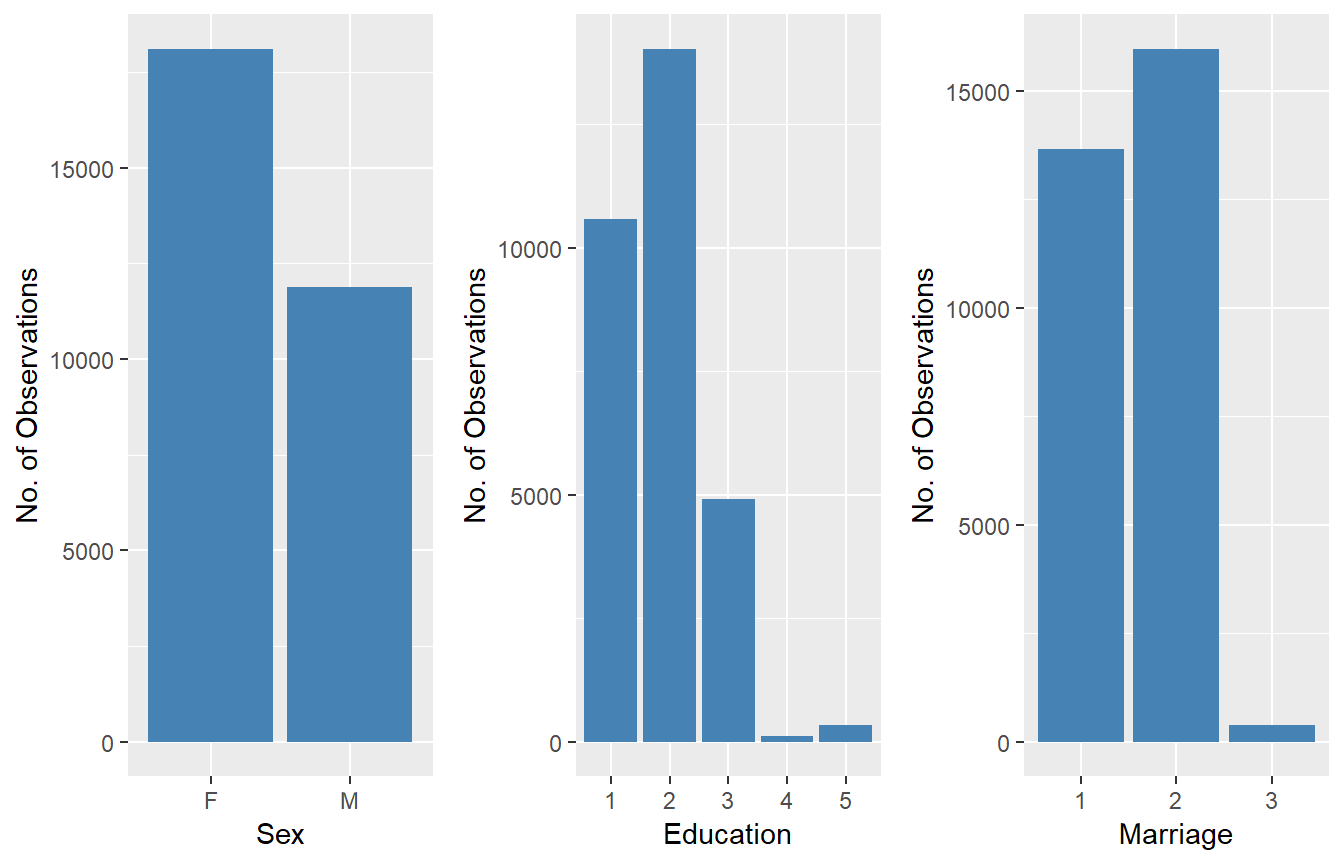
\includegraphics{TeamBlue_-_Assignment_2_files/figure-latex/unnamed-chunk-9-1.pdf}

From the above graphs we made the following observations: 1. The number
of females are more in the dataset as compared to number of males. 2.
Most of the customers achieved at least university education level. 3. A
majority of the customers is single.

Payment Status

According to the description, PAY\_x is a set of categorical variables
with the levels: -1 = pay duly 1 = payment delay for one month 2 =
payment delay for two months, ..8 = payment delay for 8 months and
9=payment delay for 9 months and above.

\begin{Shaded}
\begin{Highlighting}[]
\NormalTok{p4 =}\StringTok{ }\KeywordTok{ggplot}\NormalTok{(data,}\KeywordTok{aes}\NormalTok{(data}\OperatorTok{$}\NormalTok{PAY_STS_SEPT))}\OperatorTok{+}\KeywordTok{geom_bar}\NormalTok{(}\DataTypeTok{fill=}\StringTok{"steelblue"}\NormalTok{)}\OperatorTok{+}\KeywordTok{scale_x_discrete}\NormalTok{(}\StringTok{"Payment Status Sept_2005"}\NormalTok{)}\OperatorTok{+}\KeywordTok{scale_y_continuous}\NormalTok{(}\StringTok{"No. of Observations"}\NormalTok{)}
\NormalTok{p5 =}\StringTok{ }\KeywordTok{ggplot}\NormalTok{(data,}\KeywordTok{aes}\NormalTok{(data}\OperatorTok{$}\NormalTok{PAY_STS_AUG))}\OperatorTok{+}\KeywordTok{geom_bar}\NormalTok{(}\DataTypeTok{fill=}\StringTok{"steelblue"}\NormalTok{)}\OperatorTok{+}\KeywordTok{scale_x_discrete}\NormalTok{(}\StringTok{"Payment Status Aug_2005"}\NormalTok{)}\OperatorTok{+}\KeywordTok{scale_y_continuous}\NormalTok{(}\StringTok{"No. of Observations"}\NormalTok{)}
\NormalTok{p6 =}\StringTok{ }\KeywordTok{ggplot}\NormalTok{(data,}\KeywordTok{aes}\NormalTok{(data}\OperatorTok{$}\NormalTok{PAY_STS_JULY))}\OperatorTok{+}\KeywordTok{geom_bar}\NormalTok{(}\DataTypeTok{fill=}\StringTok{"steelblue"}\NormalTok{)}\OperatorTok{+}\KeywordTok{scale_x_discrete}\NormalTok{(}\StringTok{"Payment Status July_2005"}\NormalTok{)}\OperatorTok{+}\KeywordTok{scale_y_continuous}\NormalTok{(}\StringTok{"No. of Observations"}\NormalTok{)}
\NormalTok{p7 =}\StringTok{ }\KeywordTok{ggplot}\NormalTok{(data,}\KeywordTok{aes}\NormalTok{(data}\OperatorTok{$}\NormalTok{PAY_STS_JUNE))}\OperatorTok{+}\KeywordTok{geom_bar}\NormalTok{(}\DataTypeTok{fill=}\StringTok{"steelblue"}\NormalTok{)}\OperatorTok{+}\KeywordTok{scale_x_discrete}\NormalTok{(}\StringTok{"Payment Status June_2005"}\NormalTok{)}\OperatorTok{+}\KeywordTok{scale_y_continuous}\NormalTok{(}\StringTok{"No. of Observations"}\NormalTok{)}
\NormalTok{p8 =}\StringTok{ }\KeywordTok{ggplot}\NormalTok{(data,}\KeywordTok{aes}\NormalTok{(data}\OperatorTok{$}\NormalTok{PAY_STS_MAY))}\OperatorTok{+}\KeywordTok{geom_bar}\NormalTok{(}\DataTypeTok{fill=}\StringTok{"steelblue"}\NormalTok{)}\OperatorTok{+}\KeywordTok{scale_x_discrete}\NormalTok{(}\StringTok{"Payment Status May_2005"}\NormalTok{)}\OperatorTok{+}\KeywordTok{scale_y_continuous}\NormalTok{(}\StringTok{"No. of Observations"}\NormalTok{)}
\NormalTok{p9 =}\StringTok{ }\KeywordTok{ggplot}\NormalTok{(data,}\KeywordTok{aes}\NormalTok{(data}\OperatorTok{$}\NormalTok{PAY_STS_APRIL))}\OperatorTok{+}\KeywordTok{geom_bar}\NormalTok{(}\DataTypeTok{fill=}\StringTok{"steelblue"}\NormalTok{)}\OperatorTok{+}\KeywordTok{scale_x_discrete}\NormalTok{(}\StringTok{"Payment Status April_2005"}\NormalTok{)}\OperatorTok{+}\KeywordTok{scale_y_continuous}\NormalTok{(}\StringTok{"No. of Observations"}\NormalTok{)}
\KeywordTok{grid.arrange}\NormalTok{(p4,p5,p6,p7,p8,p9,}\DataTypeTok{nrow =} \DecValTok{2}\NormalTok{)}
\end{Highlighting}
\end{Shaded}

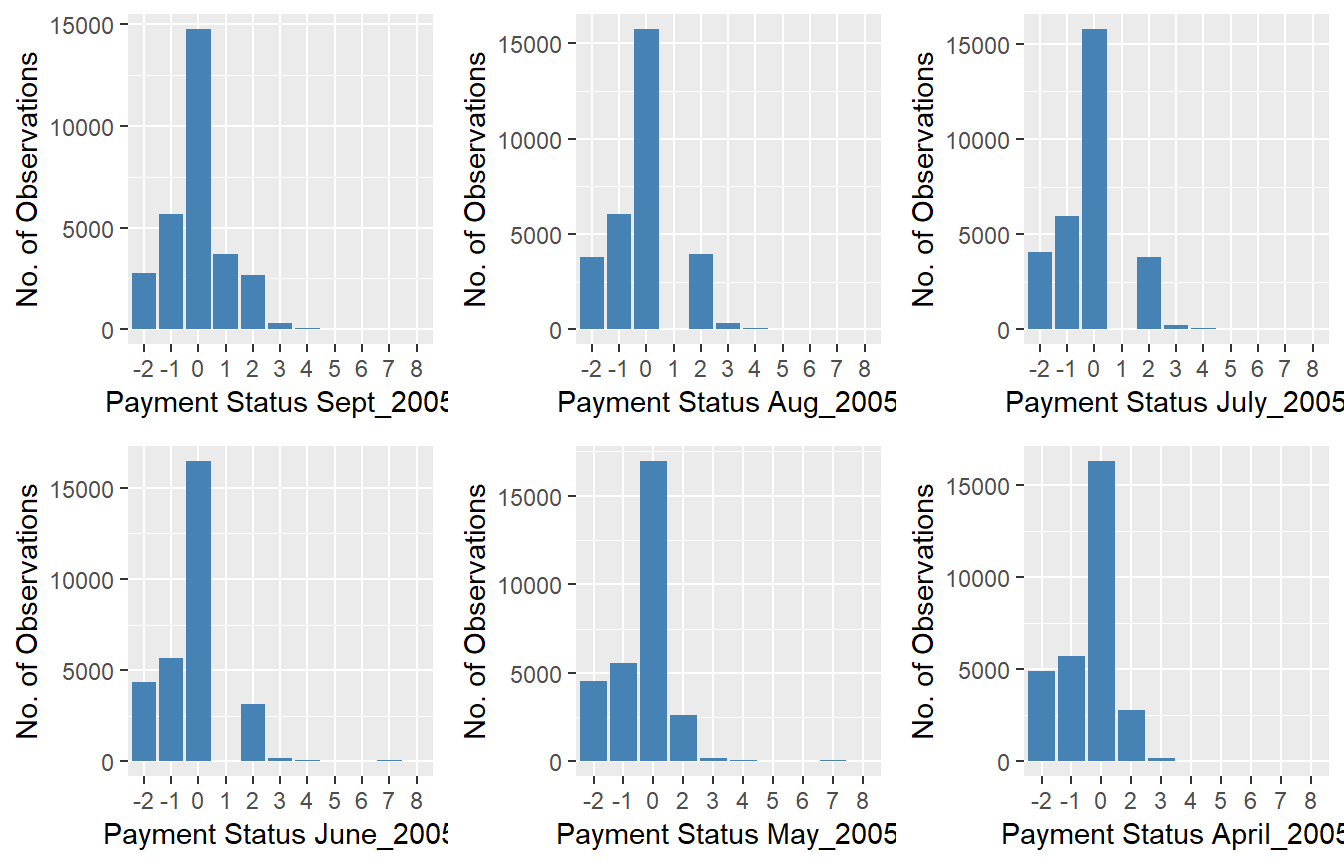
\includegraphics{TeamBlue_-_Assignment_2_files/figure-latex/unnamed-chunk-10-1.pdf}

From the above graphs we made the following observation(s): We observed
undocumented values for the PAY attributes i.e ``0'' \&``-2'' We went
back to Kaggle and searched for related discussions in the forum and we
found that these values have the following meaning. * -2 = No
consumption * 0 = The use of revolving credit card. Source:
\url{https://www.kaggle.com/uciml/default-of-credit-card-clients-dataset/discussion/34608}

So from here we found out that there are high number of observations
where people are using revolving credit card. We also observed that
there is a spike in payment delays in September 2005.

\subparagraph{Numerical Features}\label{numerical-features}

We would like to explore the distributions of the numerical variables:

Age

\begin{Shaded}
\begin{Highlighting}[]
\NormalTok{p10 =}\StringTok{ }\KeywordTok{ggplot}\NormalTok{(data, }\KeywordTok{aes}\NormalTok{(data}\OperatorTok{$}\NormalTok{AGE)) }\OperatorTok{+}\StringTok{ }\KeywordTok{geom_histogram}\NormalTok{(}\DataTypeTok{binwidth =} \DecValTok{1}\NormalTok{,}\DataTypeTok{colour=}\StringTok{"black"}\NormalTok{,}\DataTypeTok{fill=}\StringTok{"white"}\NormalTok{)}\OperatorTok{+}\StringTok{  }\KeywordTok{scale_x_continuous}\NormalTok{(}\StringTok{"Age"}\NormalTok{)}\OperatorTok{+}\KeywordTok{scale_y_continuous}\NormalTok{(}\StringTok{"Observations Count"}\NormalTok{)}\OperatorTok{+}\KeywordTok{labs}\NormalTok{(}\DataTypeTok{title =} \StringTok{"Histogram"}\NormalTok{)}
\NormalTok{p11 =}\StringTok{ }\KeywordTok{ggplot}\NormalTok{(data, }\KeywordTok{aes}\NormalTok{(,data}\OperatorTok{$}\NormalTok{AGE)) }\OperatorTok{+}\StringTok{ }\KeywordTok{geom_boxplot}\NormalTok{(}\DataTypeTok{fill =} \StringTok{"white"}\NormalTok{)}\OperatorTok{+}\StringTok{  }\KeywordTok{scale_y_continuous}\NormalTok{(}\StringTok{"Age"}\NormalTok{)}\OperatorTok{+}\KeywordTok{scale_x_continuous}\NormalTok{(}\StringTok{""}\NormalTok{)}\OperatorTok{+}\KeywordTok{labs}\NormalTok{(}\DataTypeTok{title=}\StringTok{"Boxplot"}\NormalTok{)}
\KeywordTok{grid.arrange}\NormalTok{(p10,p11,}\DataTypeTok{nrow =}\DecValTok{1}\NormalTok{,}\DataTypeTok{top=}\StringTok{"AGE DISTRIBUTION AND OUTLIERS"}\NormalTok{ )}
\end{Highlighting}
\end{Shaded}

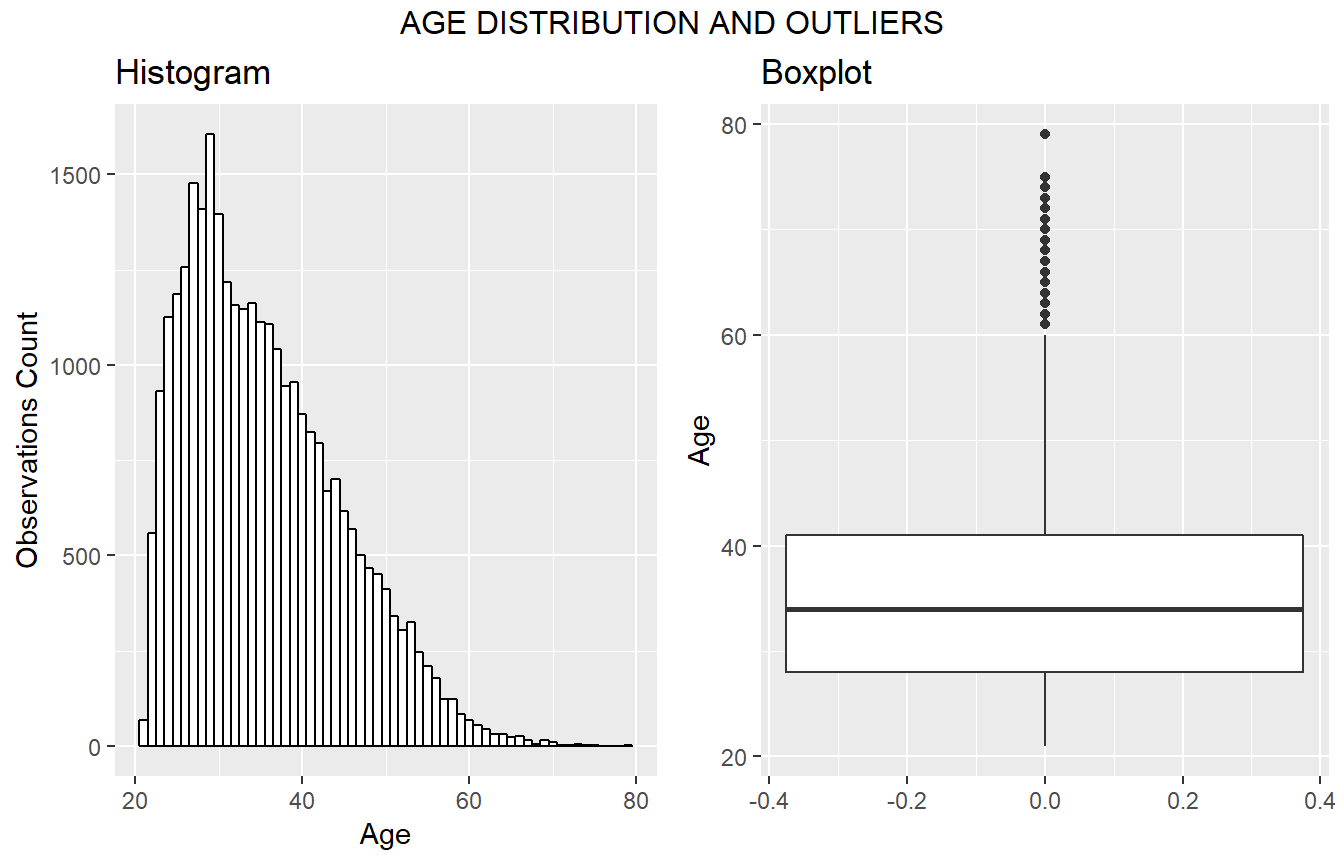
\includegraphics{TeamBlue_-_Assignment_2_files/figure-latex/unnamed-chunk-11-1.pdf}

As we can see above, the use of credit cards concentrates on younger age
(\textless{} 40) with the average age of 35.4855.

Limit of Balance

Lets explore the distribution and the outliers for the limit of balance.

\begin{Shaded}
\begin{Highlighting}[]
\KeywordTok{ggplot}\NormalTok{(data, }\KeywordTok{aes}\NormalTok{(data}\OperatorTok{$}\NormalTok{LIMIT_BAL)) }\OperatorTok{+}\StringTok{ }\KeywordTok{geom_histogram}\NormalTok{(}\DataTypeTok{binwidth =} \DecValTok{5000}\NormalTok{,}\DataTypeTok{colour=}\StringTok{"black"}\NormalTok{,}\DataTypeTok{fill=}\StringTok{"white"}\NormalTok{)}\OperatorTok{+}\StringTok{  }\KeywordTok{scale_x_continuous}\NormalTok{(}\StringTok{"Limit_BAL"}\NormalTok{)}\OperatorTok{+}\KeywordTok{scale_y_continuous}\NormalTok{(}\StringTok{"Obs."}\NormalTok{)}\OperatorTok{+}\KeywordTok{labs}\NormalTok{(}\DataTypeTok{title =} \StringTok{"Histogram"}\NormalTok{)}
\end{Highlighting}
\end{Shaded}

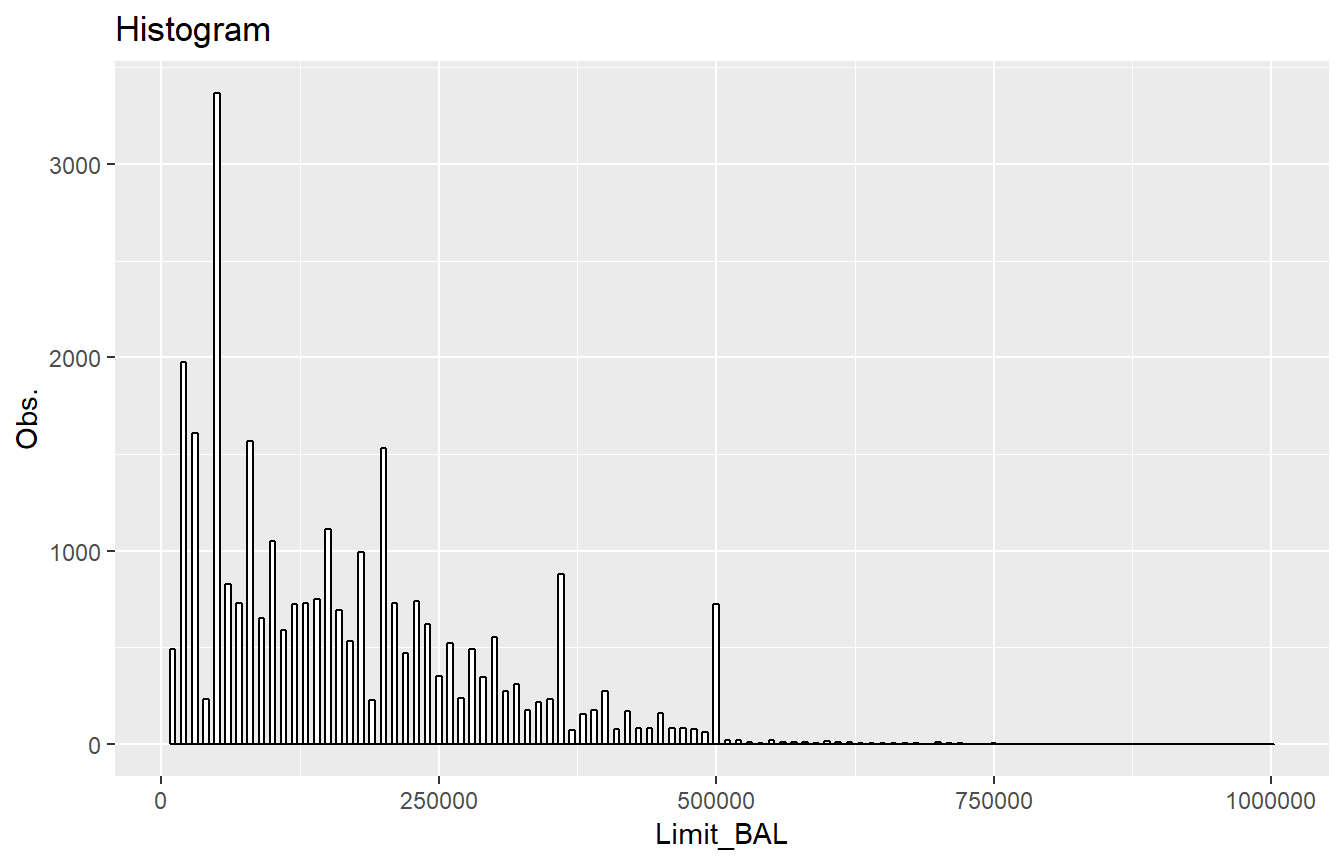
\includegraphics{TeamBlue_-_Assignment_2_files/figure-latex/unnamed-chunk-12-1.pdf}

We can see that from the above histogram, the customers usually have the
following limit balances: 20K, 30K, 50K, 80K, 200K and 500K. We also
observed that a sizable number of customers were authorized high credit
card limits above 250K.

Now lets us check for outliers with a boxplot.

\begin{Shaded}
\begin{Highlighting}[]
\KeywordTok{ggplot}\NormalTok{(data, }\KeywordTok{aes}\NormalTok{(}\DataTypeTok{x=}\KeywordTok{factor}\NormalTok{(}\DecValTok{0}\NormalTok{),}\DataTypeTok{y=}\NormalTok{data}\OperatorTok{$}\NormalTok{LIMIT_BAL)) }\OperatorTok{+}\StringTok{ }\KeywordTok{geom_boxplot}\NormalTok{(}\DataTypeTok{fill =} \StringTok{"white"}\NormalTok{)}\OperatorTok{+}
\StringTok{  }\KeywordTok{scale_y_continuous}\NormalTok{(}\StringTok{"Limit_Bal"}\NormalTok{)}\OperatorTok{+}\KeywordTok{scale_x_discrete}\NormalTok{(}\StringTok{""}\NormalTok{)}\OperatorTok{+}\KeywordTok{labs}\NormalTok{(}\DataTypeTok{title=}\StringTok{"Boxplot"}\NormalTok{)}
\end{Highlighting}
\end{Shaded}

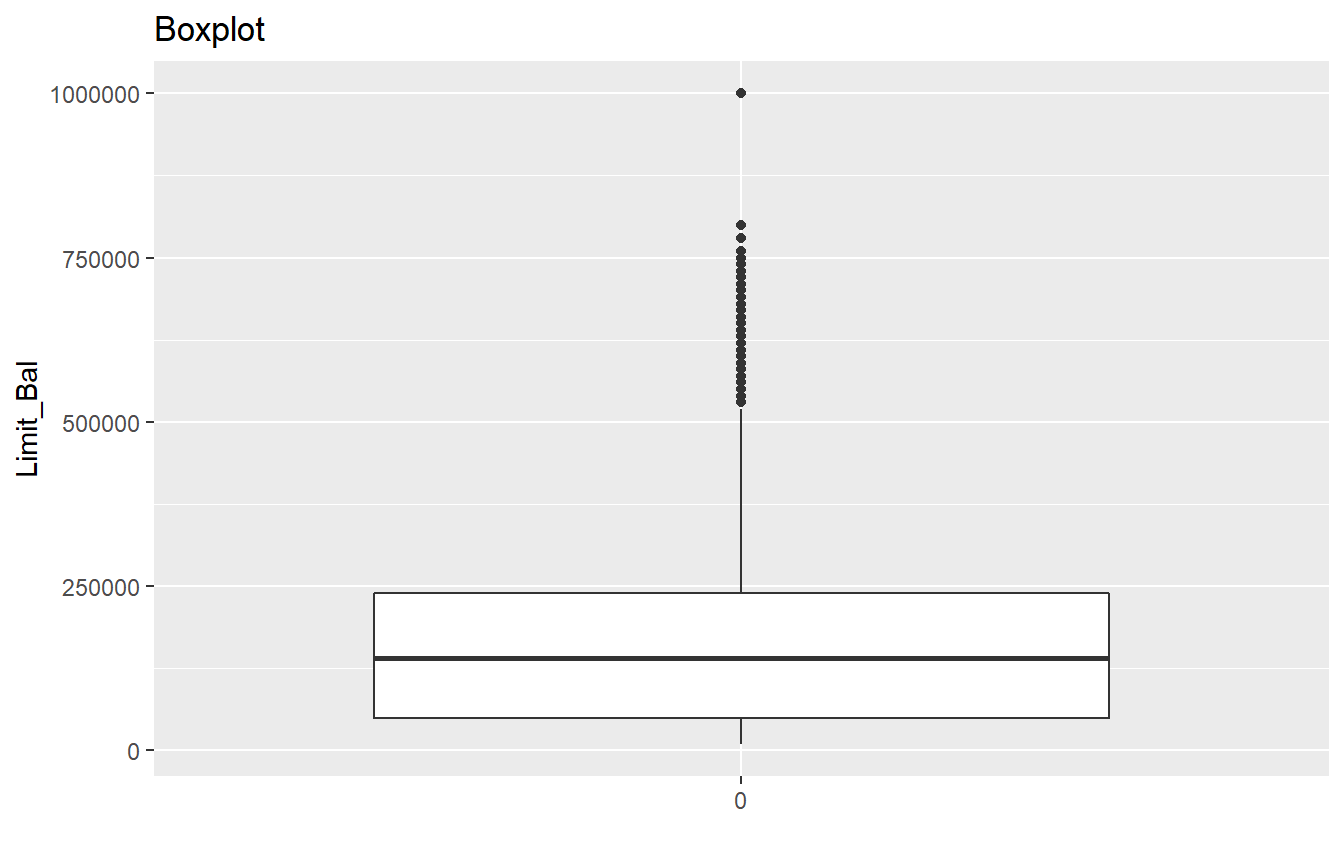
\includegraphics{TeamBlue_-_Assignment_2_files/figure-latex/unnamed-chunk-13-1.pdf}

So we can see that the 75th percentile has the credit limit of 250K.
Next we would like to know how many customers have extremely high credit
limits. We set 600K as the threshold based on the boxplot above.

\begin{Shaded}
\begin{Highlighting}[]
\NormalTok{LIMIT_BAL_OUT <-}\StringTok{ }\KeywordTok{with}\NormalTok{(data, }\KeywordTok{which}\NormalTok{(LIMIT_BAL }\OperatorTok{>}\StringTok{ }\DecValTok{600000}\NormalTok{))}
\KeywordTok{NROW}\NormalTok{(LIMIT_BAL_OUT)}
\end{Highlighting}
\end{Shaded}

\begin{verbatim}
## [1] 79
\end{verbatim}

There are 79 accounts whose limits exceed 600K. Our credit risk
monitoring team has a special monitoring program to track these accounts
because we could expose to larger losses when these customers fully draw
down the limits and then default on their debts.

Average Billing Amount \& Payment Amount.

As for the billing balances and payment amounts, since we have 6 months
of data, analyzing the balances for each month might not add much value
in the data exploring exercise. We decided to take the averages of the
billing amounts and payment amounts across the 6-month period for each
account and then observe the distributions. We will also add two columns
to populate the mean values of bill and payment amounts respectively.

\begin{Shaded}
\begin{Highlighting}[]
\NormalTok{data}\OperatorTok{$}\NormalTok{billmean <-}\StringTok{ }\KeywordTok{rowMeans}\NormalTok{(data[}\KeywordTok{c}\NormalTok{(}\StringTok{'BILL_AMT_SEPT'}\NormalTok{, }\StringTok{'BILL_AMT_AUG'}\NormalTok{,}\StringTok{'BILL_AMT_JULY'}\NormalTok{,}\StringTok{'BILL_AMT_JUNE'}\NormalTok{,}\StringTok{'BILL_AMT_MAY'}\NormalTok{,}\StringTok{'BILL_AMT_APRIL'}\NormalTok{)], }\DataTypeTok{na.rm=}\OtherTok{TRUE}\NormalTok{)}
\NormalTok{data}\OperatorTok{$}\NormalTok{paymean<-}\KeywordTok{rowMeans}\NormalTok{(data[}\KeywordTok{c}\NormalTok{(}\StringTok{'PAY_AMT_SEPT'}\NormalTok{,}\StringTok{'PAY_AMT_AUG'}\NormalTok{,}\StringTok{'PAY_AMT_JULY'}\NormalTok{,}\StringTok{'PAY_AMT_JUNE'}\NormalTok{,}\StringTok{'PAY_AMT_MAY'}\NormalTok{,}\StringTok{'PAY_AMT_APRIL'}\NormalTok{)], }\DataTypeTok{na.rm=}\OtherTok{TRUE}\NormalTok{)}
\end{Highlighting}
\end{Shaded}

Now that we have introduced the mean attributes let us plot for the
same.

\begin{Shaded}
\begin{Highlighting}[]
\NormalTok{p12 =}\StringTok{ }\KeywordTok{ggplot}\NormalTok{(data, }\KeywordTok{aes}\NormalTok{(data}\OperatorTok{$}\NormalTok{billmean)) }\OperatorTok{+}\StringTok{ }\KeywordTok{geom_histogram}\NormalTok{(}\DataTypeTok{binwidth =} \DecValTok{5000}\NormalTok{,}\DataTypeTok{colour=}\StringTok{"black"}\NormalTok{,}\DataTypeTok{fill=}\StringTok{"white"}\NormalTok{)}\OperatorTok{+}\StringTok{  }\KeywordTok{scale_x_continuous}\NormalTok{(}\StringTok{"Mean Bill Amount"}\NormalTok{)}\OperatorTok{+}\KeywordTok{scale_y_continuous}\NormalTok{(}\StringTok{"Obs."}\NormalTok{)}
\NormalTok{p24 =}\StringTok{ }\KeywordTok{ggplot}\NormalTok{(data, }\KeywordTok{aes}\NormalTok{(data}\OperatorTok{$}\NormalTok{paymean)) }\OperatorTok{+}\StringTok{ }\KeywordTok{geom_histogram}\NormalTok{(}\DataTypeTok{binwidth =} \DecValTok{5000}\NormalTok{,}\DataTypeTok{colour=}\StringTok{"black"}\NormalTok{,}\DataTypeTok{fill=}\StringTok{"white"}\NormalTok{)}\OperatorTok{+}\StringTok{  }\KeywordTok{scale_x_continuous}\NormalTok{(}\StringTok{"Mean Payment Amount"}\NormalTok{)}\OperatorTok{+}\KeywordTok{scale_y_continuous}\NormalTok{(}\StringTok{"Obs."}\NormalTok{)}
\KeywordTok{grid.arrange}\NormalTok{(p12,p24,}\DataTypeTok{nrow=}\DecValTok{1}\NormalTok{,}\DataTypeTok{top =} \StringTok{"Avergae Bill & Payment amount for all months"}\NormalTok{)}
\end{Highlighting}
\end{Shaded}

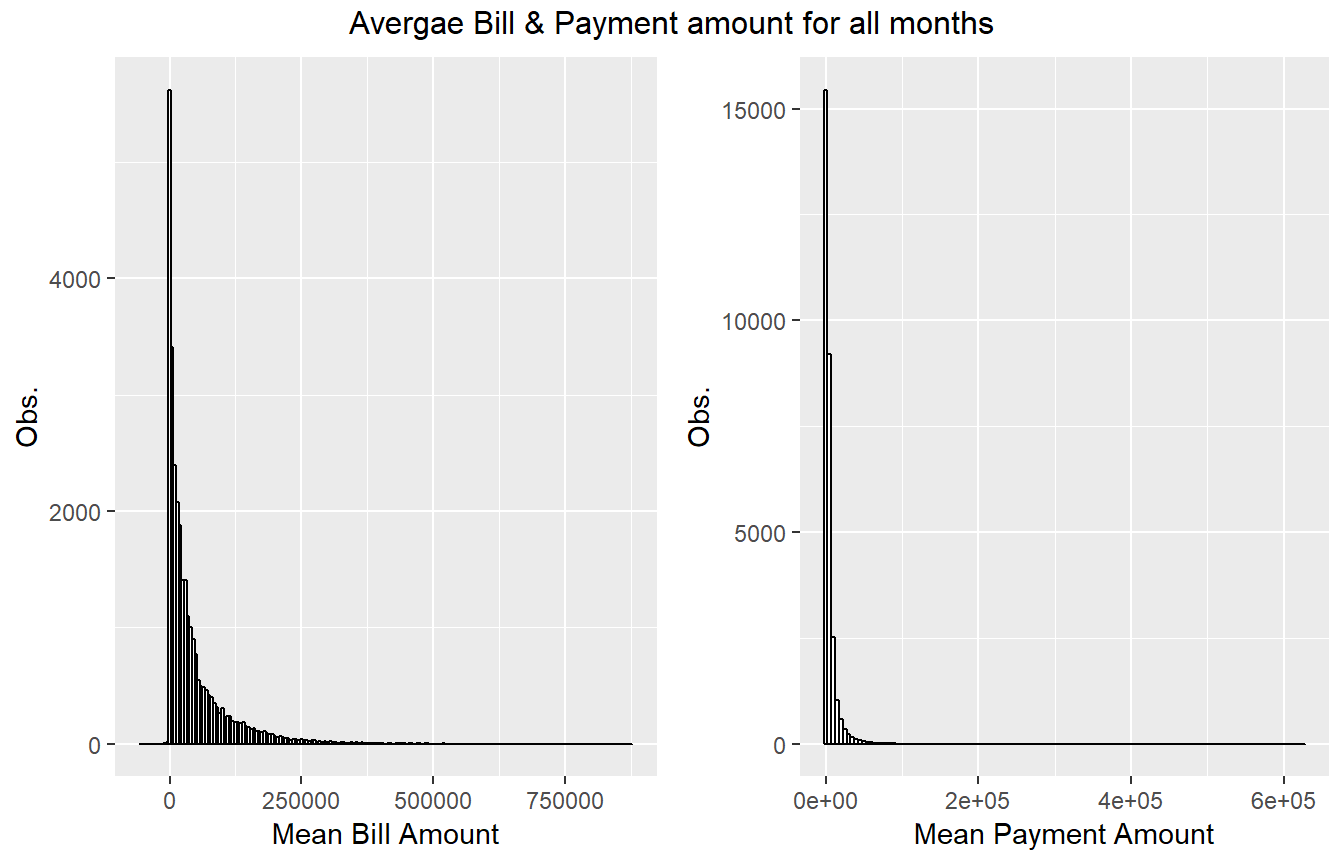
\includegraphics{TeamBlue_-_Assignment_2_files/figure-latex/unnamed-chunk-16-1.pdf}

Based on the above charts, we observe that the customers tend to pay off
the credit cards bills in smaller amounts than the actual amounts in the
bill statements as the distribution of the payment amounts are very
skewed towards smaller values. The disbution of the bill amounts is also
skewed but it has fatter tail at the high bill amount area.

The skewness of these distributions can be further visualized in the
boxplots below:

\begin{Shaded}
\begin{Highlighting}[]
\NormalTok{p18 =}\StringTok{ }\KeywordTok{ggplot}\NormalTok{(data, }\KeywordTok{aes}\NormalTok{(,data}\OperatorTok{$}\NormalTok{billmean)) }\OperatorTok{+}\StringTok{ }\KeywordTok{geom_boxplot}\NormalTok{(}\DataTypeTok{fill =} \StringTok{"white"}\NormalTok{)}\OperatorTok{+}\StringTok{ }\KeywordTok{scale_y_continuous}\NormalTok{(}\StringTok{"Average Billing Amount"}\NormalTok{)}\OperatorTok{+}\KeywordTok{scale_x_continuous}\NormalTok{(}\StringTok{""}\NormalTok{)}
\NormalTok{p30 =}\StringTok{ }\KeywordTok{ggplot}\NormalTok{(data, }\KeywordTok{aes}\NormalTok{(,data}\OperatorTok{$}\NormalTok{paymean)) }\OperatorTok{+}\StringTok{ }\KeywordTok{geom_boxplot}\NormalTok{(}\DataTypeTok{fill =} \StringTok{"white"}\NormalTok{)}\OperatorTok{+}\StringTok{  }\KeywordTok{scale_y_continuous}\NormalTok{(}\StringTok{"Average Payment Amount"}\NormalTok{)}\OperatorTok{+}\KeywordTok{scale_x_continuous}\NormalTok{(}\StringTok{""}\NormalTok{)}
\KeywordTok{grid.arrange}\NormalTok{(p18,p30,}\DataTypeTok{ncol=}\DecValTok{2}\NormalTok{,}\DataTypeTok{top=}\StringTok{"Boxplot for Avergae Bill & Payment amount for all months"}\NormalTok{)}
\end{Highlighting}
\end{Shaded}

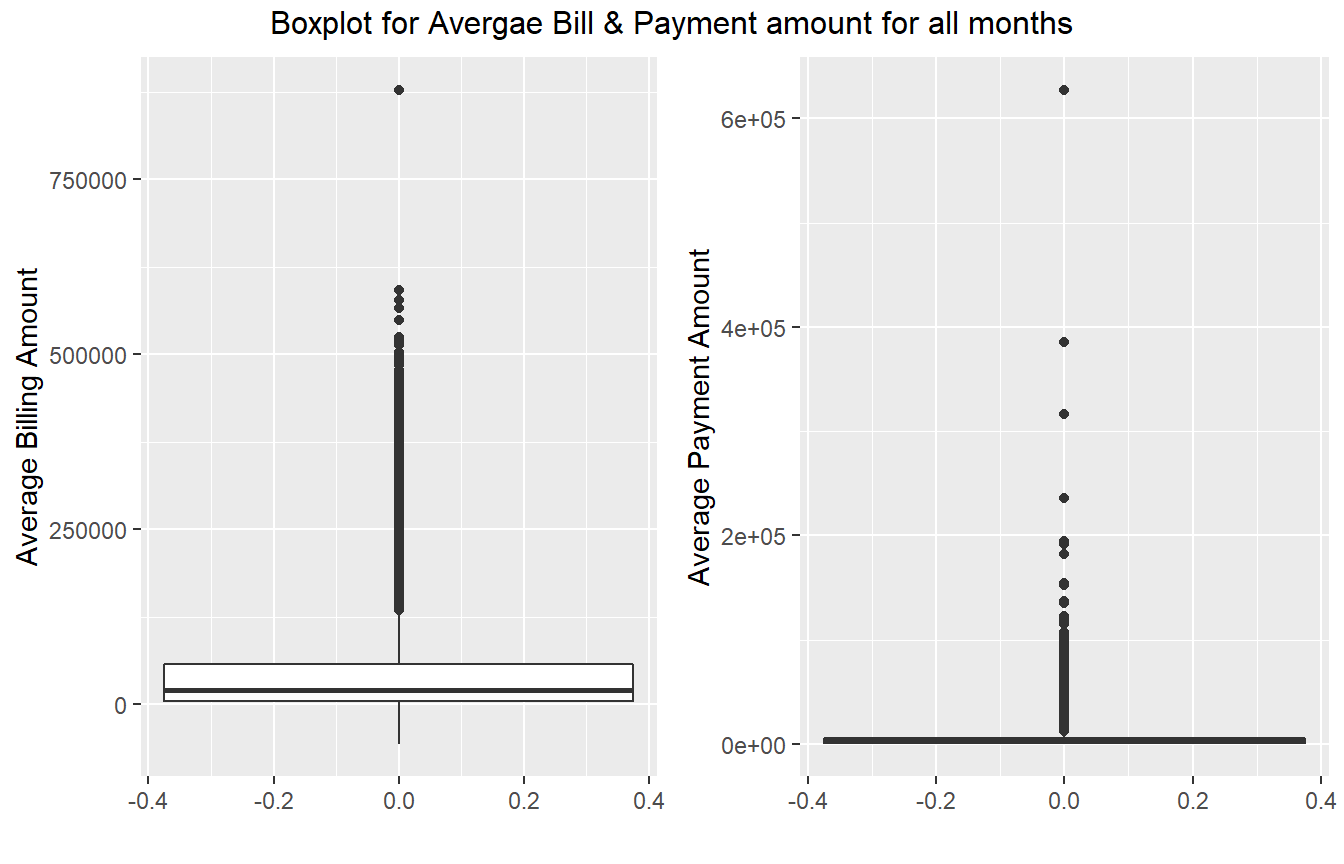
\includegraphics{TeamBlue_-_Assignment_2_files/figure-latex/unnamed-chunk-17-1.pdf}

Once again, the boxplots verify our observations above.

\paragraph{Bivariate Exploration}\label{bivariate-exploration}

We will look at the following relationships in the dataset:

\begin{itemize}
\tightlist
\item
  Marriage Status and Repayment Status
\item
  Sex and Repayment Status
\item
  Education and Repayment Status
\end{itemize}

\subparagraph{Marriage status and Repayment
Status}\label{marriage-status-and-repayment-status}

We are using the repayment data as of Seotember 2005 for us to draw the
insights.

Let us take a look at the relationship between marriage status and
re-payment status as of September 2005:

\begin{Shaded}
\begin{Highlighting}[]
\KeywordTok{ggplot}\NormalTok{(data,}\KeywordTok{aes}\NormalTok{(}\DataTypeTok{x=}\NormalTok{PAY_STS_SEPT,}\DataTypeTok{fill =}\NormalTok{ MARRIAGE))}\OperatorTok{+}\KeywordTok{geom_bar}\NormalTok{(}\DataTypeTok{position =} \StringTok{"fill"}\NormalTok{)}\OperatorTok{+}\KeywordTok{scale_x_discrete}\NormalTok{(}\StringTok{"Repayment Status in September 2005"}\NormalTok{)}
\end{Highlighting}
\end{Shaded}

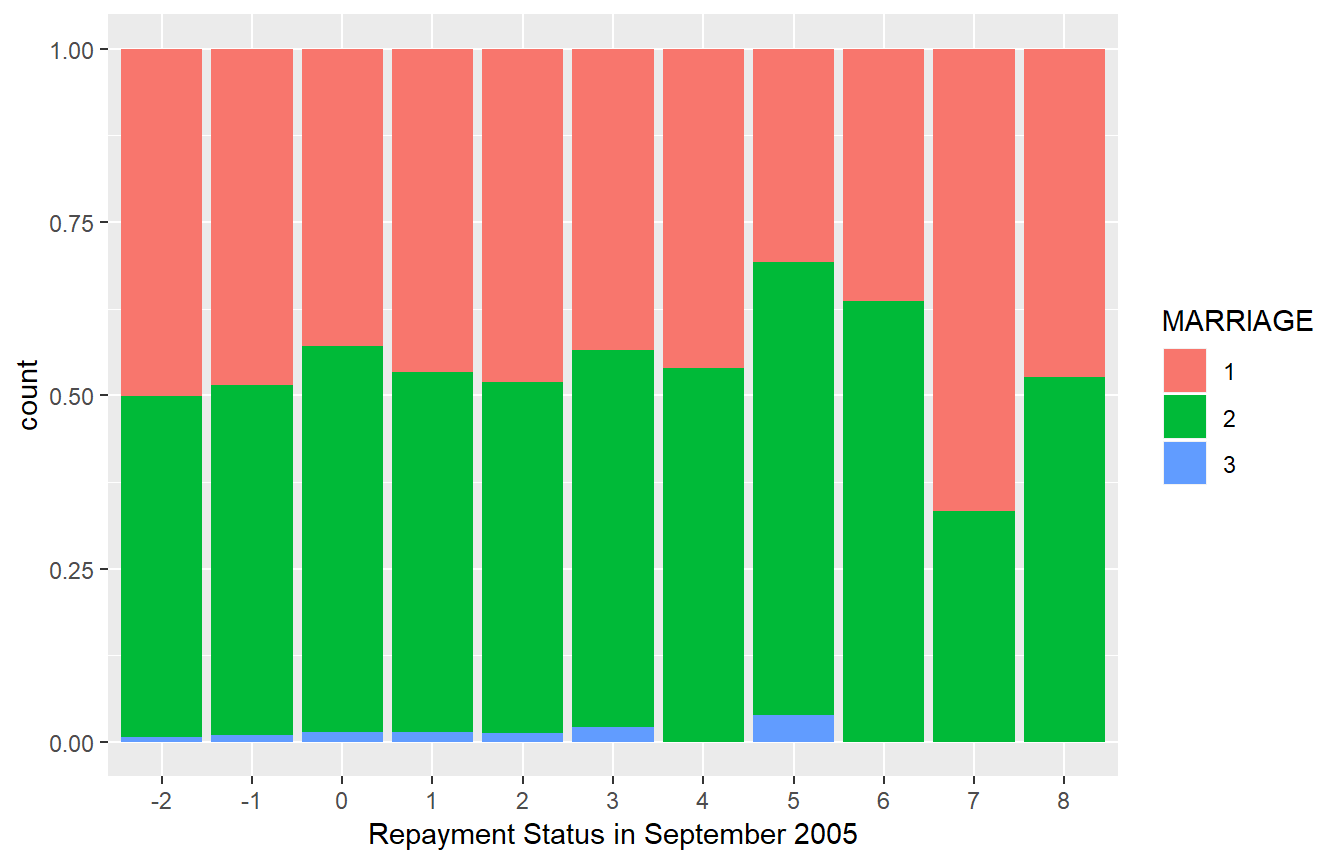
\includegraphics{TeamBlue_-_Assignment_2_files/figure-latex/unnamed-chunk-18-1.pdf}

To recap, here is the description of the repayment status flag: (-1=pay
duly, 1=payment delay for one month, 2=payment delay for two months,
\ldots{} 8=payment delay for eight months, 9=payment delay for nine
months and above)

Based on the chart above, we observe that majority of the customers who
are behind on their credit card payments are mostly single, except the
7-month delay bucket.

\subparagraph{Sex and Repayment Status}\label{sex-and-repayment-status}

Now lets check if there is any trend we can observe if we plot the
repayment status w.r.t gender.

\begin{Shaded}
\begin{Highlighting}[]
\KeywordTok{ggplot}\NormalTok{(data,}\KeywordTok{aes}\NormalTok{(}\DataTypeTok{x=}\NormalTok{PAY_STS_SEPT,}\DataTypeTok{fill =}\NormalTok{ SEX))}\OperatorTok{+}\KeywordTok{geom_bar}\NormalTok{(}\DataTypeTok{position =} \StringTok{"fill"}\NormalTok{)}\OperatorTok{+}\KeywordTok{scale_x_discrete}\NormalTok{(}\StringTok{"Repayment Status in September 2005"}\NormalTok{)}
\end{Highlighting}
\end{Shaded}

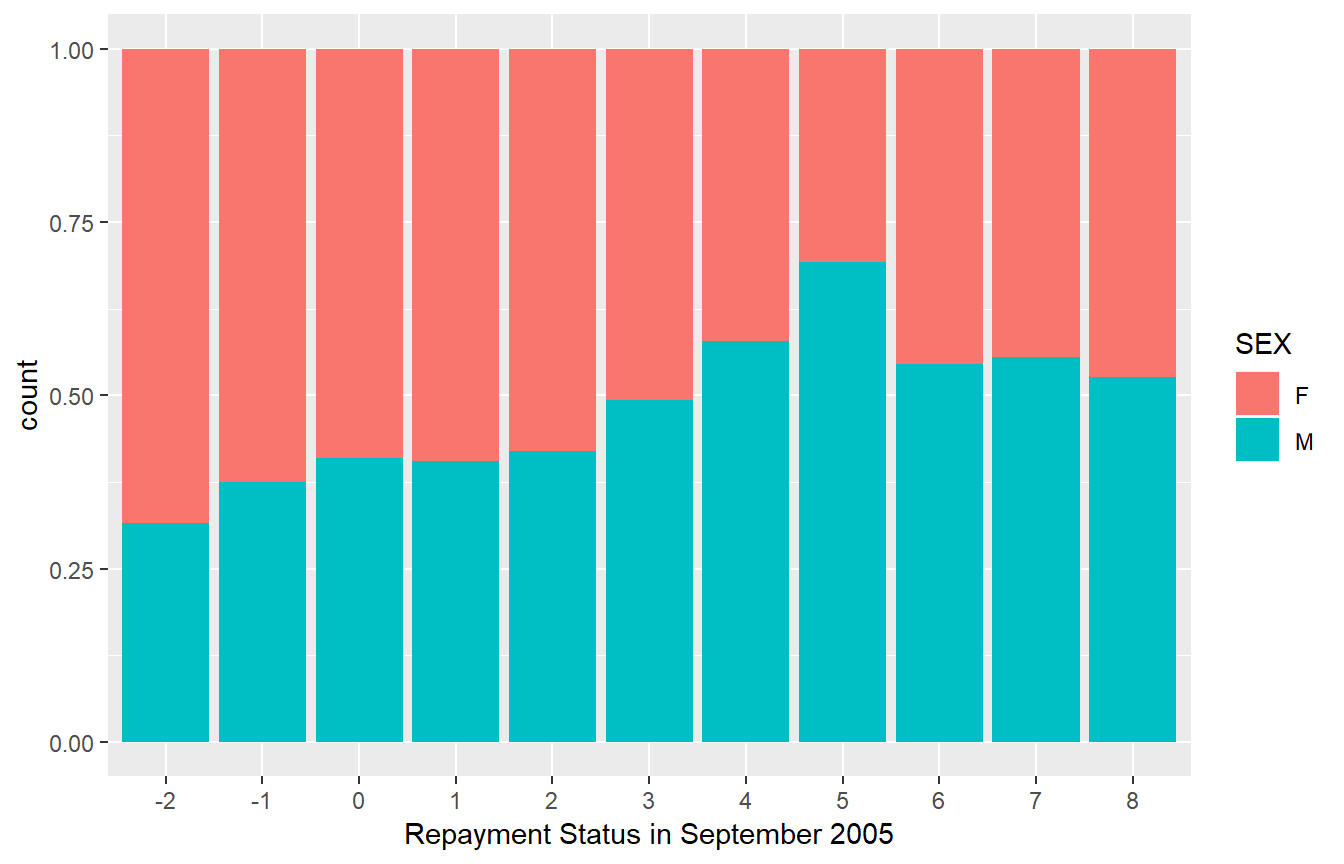
\includegraphics{TeamBlue_-_Assignment_2_files/figure-latex/unnamed-chunk-19-1.pdf}

We observed that a majority of customers who is behind on their credit
card payments is male as of September 2005.

Let us check for the rest of the months to see if it is the same
situation every month.

\begin{Shaded}
\begin{Highlighting}[]
\NormalTok{b1 =}\StringTok{ }\KeywordTok{ggplot}\NormalTok{(data,}\KeywordTok{aes}\NormalTok{(}\DataTypeTok{x=}\NormalTok{PAY_STS_AUG,}\DataTypeTok{fill =}\NormalTok{ SEX))}\OperatorTok{+}\KeywordTok{geom_bar}\NormalTok{(}\DataTypeTok{position =} \StringTok{"fill"}\NormalTok{)}\OperatorTok{+}\KeywordTok{scale_x_discrete}\NormalTok{(}\StringTok{"Repayment Status in August 2005"}\NormalTok{)}
\NormalTok{b2 =}\StringTok{ }\KeywordTok{ggplot}\NormalTok{(data,}\KeywordTok{aes}\NormalTok{(}\DataTypeTok{x=}\NormalTok{PAY_STS_JULY,}\DataTypeTok{fill =}\NormalTok{ SEX))}\OperatorTok{+}\KeywordTok{geom_bar}\NormalTok{(}\DataTypeTok{position =} \StringTok{"fill"}\NormalTok{)}\OperatorTok{+}\KeywordTok{scale_x_discrete}\NormalTok{(}\StringTok{"Repayment Status in July 2005"}\NormalTok{)}
\NormalTok{b3 =}\StringTok{ }\KeywordTok{ggplot}\NormalTok{(data,}\KeywordTok{aes}\NormalTok{(}\DataTypeTok{x=}\NormalTok{PAY_STS_JUNE,}\DataTypeTok{fill =}\NormalTok{ SEX))}\OperatorTok{+}\KeywordTok{geom_bar}\NormalTok{(}\DataTypeTok{position =} \StringTok{"fill"}\NormalTok{)}\OperatorTok{+}\KeywordTok{scale_x_discrete}\NormalTok{(}\StringTok{"Repayment Status in June 2005"}\NormalTok{)}
\NormalTok{b4 =}\StringTok{ }\KeywordTok{ggplot}\NormalTok{(data,}\KeywordTok{aes}\NormalTok{(}\DataTypeTok{x=}\NormalTok{PAY_STS_MAY,}\DataTypeTok{fill =}\NormalTok{ SEX))}\OperatorTok{+}\KeywordTok{geom_bar}\NormalTok{(}\DataTypeTok{position =} \StringTok{"fill"}\NormalTok{)}\OperatorTok{+}\KeywordTok{scale_x_discrete}\NormalTok{(}\StringTok{"Repayment Status in May 2005"}\NormalTok{)}
\NormalTok{b5 =}\StringTok{ }\KeywordTok{ggplot}\NormalTok{(data,}\KeywordTok{aes}\NormalTok{(}\DataTypeTok{x=}\NormalTok{PAY_STS_APRIL,}\DataTypeTok{fill =}\NormalTok{ SEX))}\OperatorTok{+}\KeywordTok{geom_bar}\NormalTok{(}\DataTypeTok{position =} \StringTok{"fill"}\NormalTok{)}\OperatorTok{+}\KeywordTok{scale_x_discrete}\NormalTok{(}\StringTok{"Repayment Status in April 2005"}\NormalTok{)}
\KeywordTok{grid.arrange}\NormalTok{(b1,b2,b3,b4,b5,}\DataTypeTok{nrow =} \DecValTok{3}\NormalTok{)}
\end{Highlighting}
\end{Shaded}

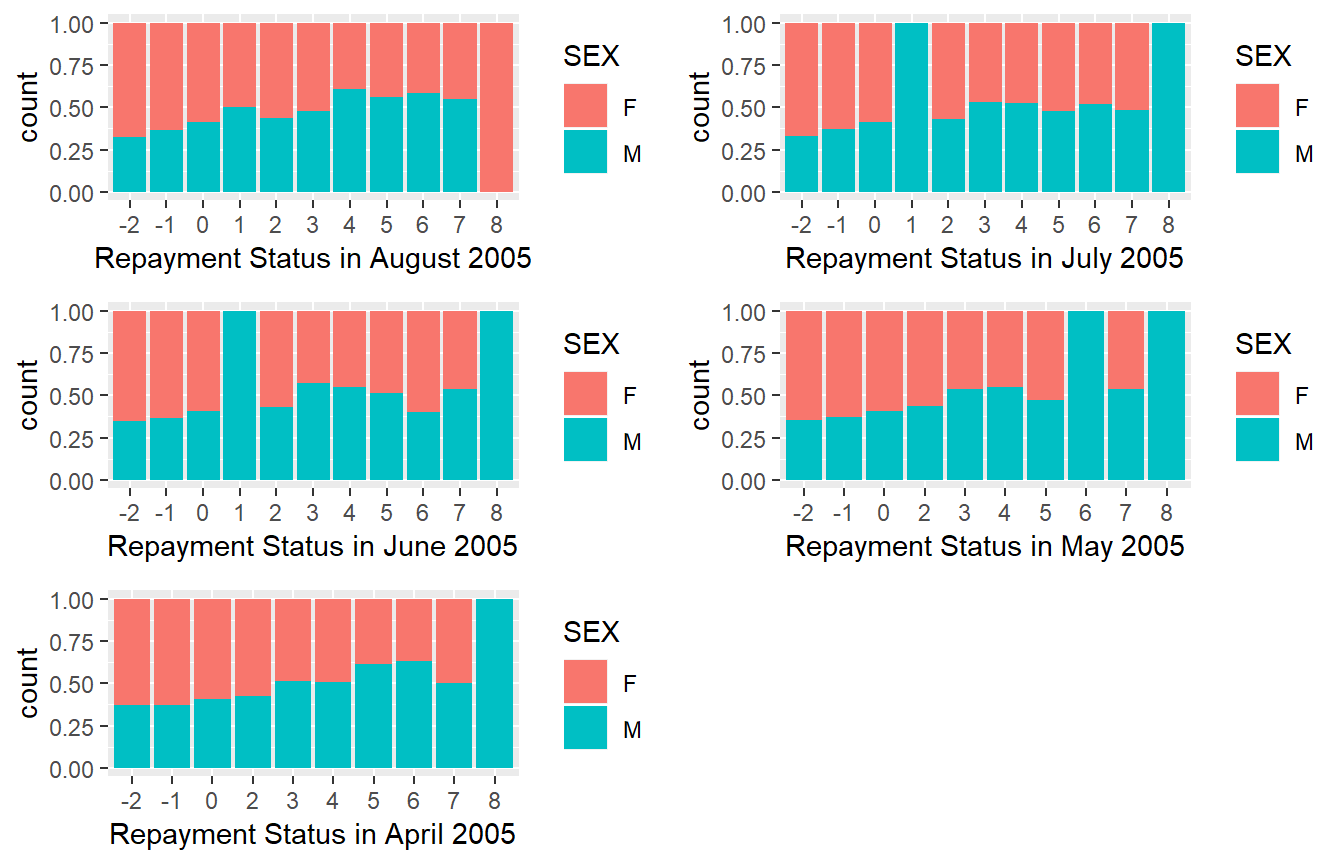
\includegraphics{TeamBlue_-_Assignment_2_files/figure-latex/unnamed-chunk-20-1.pdf}

Just as we suspected! The males are more likely to be behind their
credit card bills.

\subparagraph{Education and Repayment
Status}\label{education-and-repayment-status}

\begin{Shaded}
\begin{Highlighting}[]
\KeywordTok{ggplot}\NormalTok{(data,}\KeywordTok{aes}\NormalTok{(}\DataTypeTok{x=}\NormalTok{PAY_STS_SEPT,}\DataTypeTok{fill =}\NormalTok{ EDUCATION))}\OperatorTok{+}\KeywordTok{geom_bar}\NormalTok{(}\DataTypeTok{position =} \StringTok{"fill"}\NormalTok{)}\OperatorTok{+}\KeywordTok{scale_x_discrete}\NormalTok{(}\StringTok{"Repayment Status in September 2005"}\NormalTok{)}
\end{Highlighting}
\end{Shaded}

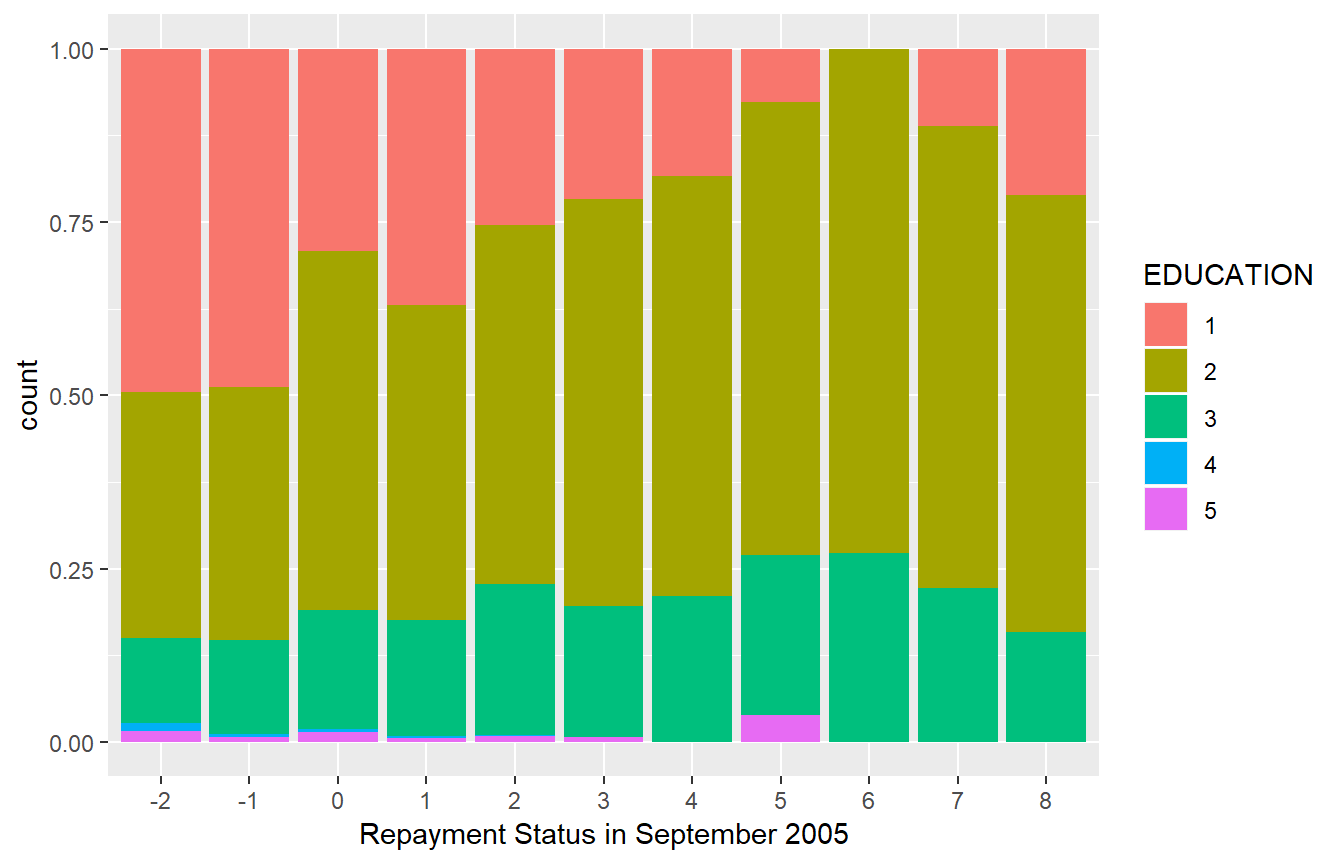
\includegraphics{TeamBlue_-_Assignment_2_files/figure-latex/unnamed-chunk-21-1.pdf}

To recap, here is the description of the repayment status flag: (-1=pay
duly, 1=payment delay for one month, 2=payment delay for two months,
\ldots{} 8=payment delay for eight months, 9=payment delay for nine
months and above). The education level flag has the following legend:
(1=graduate school, 2=university, 3=high school, 4=others, 5=unknown)

We observe that most customers who are behind their credit card payments
have at least univerity education. Since the observation is most likely
the same for the other months, we won't repeat the analysus here.

\section{DATA PREPARATION}\label{data-preparation}

\subsection{Check for missing values.}\label{check-for-missing-values.}

Now that we have explored the original data lets look for missing
values.

\begin{Shaded}
\begin{Highlighting}[]
\KeywordTok{sum}\NormalTok{(}\KeywordTok{is.na.data.frame}\NormalTok{(data))}
\end{Highlighting}
\end{Shaded}

\begin{verbatim}
## [1] 0
\end{verbatim}

So we can see from above that we have 0 missing values so we don't have
to fill in missing values.

\subsection{Data Cleaning}\label{data-cleaning}

Earlier we had introduced two new attributes (billmean \& paymean) for
our data explorations. We will now remove them as we don't need them in
our modelling work.

\begin{Shaded}
\begin{Highlighting}[]
\NormalTok{data}\OperatorTok{$}\NormalTok{billmean<-}\OtherTok{NULL}
\NormalTok{data}\OperatorTok{$}\NormalTok{paymean<-}\OtherTok{NULL}
\end{Highlighting}
\end{Shaded}

\subsection{Create Payment Ratios}\label{create-payment-ratios}

Let's look at the relationship between the Bill\_AMT{[}N{]} and
Pay\_AMT{[}N{]} variables, where N is from September to April 2005.
Normally, a bill statement is issued in the month after the payment
month. That is, for example, a customer receives the statement in July
2005 in which the customer is required to clear the balance in August
2005.

\begin{Shaded}
\begin{Highlighting}[]
\NormalTok{data[}\DecValTok{1}\NormalTok{,}\KeywordTok{colnames}\NormalTok{(data) }\OperatorTok\StringTok{ }\KeywordTok{c}\NormalTok{(}\StringTok{"BILL_AMT_JULY"}\NormalTok{,}\StringTok{"PAY_AMT_AUG"}\NormalTok{)]}
\end{Highlighting}
\end{Shaded}

\begin{verbatim}
##   BILL_AMT_JULY PAY_AMT_AUG
## 1           689         689
\end{verbatim}

We created ratios to see how much of the previous month bill did the
user pay off. We made some assumptions where if the Bill Amount is
negative then the ratio should be 1 has the bill has been overpaid.

\begin{Shaded}
\begin{Highlighting}[]
\NormalTok{data}\OperatorTok{$}\NormalTok{Ratio_BILL_AUG <-}\StringTok{ }\KeywordTok{ifelse}\NormalTok{(data}\OperatorTok{$}\NormalTok{PAY_AMT_SEPT}\OperatorTok{==}\DecValTok{0}\NormalTok{,}\DecValTok{0}\NormalTok{,}\KeywordTok{ifelse}\NormalTok{(data}\OperatorTok{$}\NormalTok{BILL_AMT_AUG }\OperatorTok{<=}\DecValTok{0}\NormalTok{,}\DecValTok{1}\NormalTok{,data}\OperatorTok{$}\NormalTok{PAY_AMT_SEPT}\OperatorTok{/}\NormalTok{data}\OperatorTok{$}\NormalTok{BILL_AMT_AUG))}
\NormalTok{data}\OperatorTok{$}\NormalTok{Ratio_BILL_JULY <-}\StringTok{ }\KeywordTok{ifelse}\NormalTok{(data}\OperatorTok{$}\NormalTok{PAY_AMT_AUG}\OperatorTok{==}\DecValTok{0}\NormalTok{,}\DecValTok{0}\NormalTok{,}\KeywordTok{ifelse}\NormalTok{(data}\OperatorTok{$}\NormalTok{BILL_AMT_JULY }\OperatorTok{<=}\DecValTok{0}\NormalTok{,}\DecValTok{1}\NormalTok{,data}\OperatorTok{$}\NormalTok{PAY_AMT_AUG}\OperatorTok{/}\NormalTok{data}\OperatorTok{$}\NormalTok{BILL_AMT_JULY))}
\NormalTok{data}\OperatorTok{$}\NormalTok{Ratio_BILL_JUNE <-}\StringTok{ }\KeywordTok{ifelse}\NormalTok{(data}\OperatorTok{$}\NormalTok{PAY_AMT_JULY}\OperatorTok{==}\DecValTok{0}\NormalTok{,}\DecValTok{0}\NormalTok{,}\KeywordTok{ifelse}\NormalTok{(data}\OperatorTok{$}\NormalTok{BILL_AMT_JUNE }\OperatorTok{<=}\DecValTok{0}\NormalTok{,}\DecValTok{1}\NormalTok{,data}\OperatorTok{$}\NormalTok{PAY_AMT_JULY}\OperatorTok{/}\NormalTok{data}\OperatorTok{$}\NormalTok{BILL_AMT_JUNE))}
\NormalTok{data}\OperatorTok{$}\NormalTok{Ratio_BILL_MAY <-}\StringTok{ }\KeywordTok{ifelse}\NormalTok{(data}\OperatorTok{$}\NormalTok{PAY_AMT_JUNE}\OperatorTok{==}\DecValTok{0}\NormalTok{,}\DecValTok{0}\NormalTok{,}\KeywordTok{ifelse}\NormalTok{(data}\OperatorTok{$}\NormalTok{BILL_AMT_MAY }\OperatorTok{<=}\DecValTok{0}\NormalTok{,}\DecValTok{1}\NormalTok{,data}\OperatorTok{$}\NormalTok{PAY_AMT_JUNE}\OperatorTok{/}\NormalTok{data}\OperatorTok{$}\NormalTok{BILL_AMT_MAY))}
\NormalTok{data}\OperatorTok{$}\NormalTok{Ratio_BILL_APRIL <-}\StringTok{ }\KeywordTok{ifelse}\NormalTok{(data}\OperatorTok{$}\NormalTok{PAY_AMT_MAY}\OperatorTok{==}\DecValTok{0}\NormalTok{,}\DecValTok{0}\NormalTok{,}\KeywordTok{ifelse}\NormalTok{(data}\OperatorTok{$}\NormalTok{BILL_AMT_APRIL }\OperatorTok{<=}\DecValTok{0}\NormalTok{,}\DecValTok{1}\NormalTok{,data}\OperatorTok{$}\NormalTok{PAY_AMT_MAY}\OperatorTok{/}\NormalTok{data}\OperatorTok{$}\NormalTok{BILL_AMT_APRIL))}
\end{Highlighting}
\end{Shaded}

\section{Modelling}\label{modelling}

\subsection{Select Modelling
Technique}\label{select-modelling-technique}

We chose to start with a K means clustering alorgirthm as most of our
data are numeric. The first step for running the alogirthm is to make
all the categorical variables into numeric by encoding them. We chose to
implement one hot encoding because our variables are nominal and not
ordinal.

\subsection{Encode Data}\label{encode-data}

\begin{Shaded}
\begin{Highlighting}[]
\NormalTok{data_f <-}\StringTok{ }\NormalTok{data}

\CommentTok{#encod categorical columns}
\NormalTok{dummies_model <-}\StringTok{ }\KeywordTok{dummyVars}\NormalTok{(ï..ID }\OperatorTok{~}\StringTok{ }\NormalTok{., }\DataTypeTok{data=}\NormalTok{data_f)}

\CommentTok{# Create the dummy variables using predict. The Y variable (ï..ID) will not be present in encod}
\NormalTok{encod <-}\StringTok{ }\KeywordTok{predict}\NormalTok{(dummies_model, }\DataTypeTok{newdata =}\NormalTok{ data_f)}

\CommentTok{# # Convert to dataframe}
\NormalTok{data_encoded <-}\StringTok{ }\KeywordTok{data.frame}\NormalTok{(encod)}

\CommentTok{# # Summary of the new dataset}
\CommentTok{#str(data_encoded)}
\end{Highlighting}
\end{Shaded}

Now that the data is encoded and all variables are numeric, we can
implement the K means algorithm. The K means algorithm works by creating
K cluster. Each cluster is based on feature similarity. The alogirthm
starts by randomly picking K centroids, then the alogirthm iterates
through each point and assigns it to the nearest cluster based a
distance formula. (ex: Euclidean). After each point has been assigned a
cluster, the centroids are re-calculated by taking the mean distances of
all data points in the clusters, next the points are reclassifed again
until a stopping criteria is met. (No points change clusters or the mean
of all data points in the cluster is minimized.)

\subsection{Normalize the Data}\label{normalize-the-data}

Since the K means algorithm using distance to find the nearest point we
need to ensure all the variables are on the same range. We do this by
normalizing the data.

\begin{Shaded}
\begin{Highlighting}[]
\NormalTok{df <-}\StringTok{ }\NormalTok{data_encoded}

\NormalTok{normalize =}\StringTok{ }\ControlFlowTok{function}\NormalTok{(x) \{}
  \KeywordTok{return}\NormalTok{ ((x }\OperatorTok{-}\StringTok{ }\KeywordTok{min}\NormalTok{(x)) }\OperatorTok{/}\StringTok{ }\NormalTok{(}\KeywordTok{max}\NormalTok{(x) }\OperatorTok{-}\StringTok{ }\KeywordTok{min}\NormalTok{(x)))}
\NormalTok{\}}

\NormalTok{df =}\StringTok{ }\KeywordTok{as.data.frame}\NormalTok{(}\KeywordTok{lapply}\NormalTok{(df, normalize))}
\end{Highlighting}
\end{Shaded}

\subsection{Find Optimal Number of Clusters
(K)}\label{find-optimal-number-of-clusters-k}

Before we run the K Mean algorithm we need to find the optimal K
clusters. To find the optimal number of clusters we used the Elbow
method. The elbow method finds the optimal K value by running mulptiple
K Means for K from 1 to N and calculateing the Sum of Squared errors
(SSE). We then plot each SSE for each K, we then chose an optimal value
of K such that it has a low SSE but further increase of K would make
little improvement to the SSE. That K value would be the elbow point of
the plot.

\begin{Shaded}
\begin{Highlighting}[]
\CommentTok{#Find Optimal K using Elbow method}

\NormalTok{wssplot <-}\StringTok{ }\ControlFlowTok{function}\NormalTok{(data, }\DataTypeTok{nc=}\DecValTok{15}\NormalTok{, }\DataTypeTok{seed=}\DecValTok{1234}\NormalTok{)\{}
\NormalTok{  wss <-}\StringTok{ }\NormalTok{(}\KeywordTok{nrow}\NormalTok{(data)}\OperatorTok{-}\DecValTok{1}\NormalTok{)}\OperatorTok{*}\KeywordTok{sum}\NormalTok{(}\KeywordTok{apply}\NormalTok{(data,}\DecValTok{2}\NormalTok{,var))}
  \ControlFlowTok{for}\NormalTok{ (i }\ControlFlowTok{in} \DecValTok{2}\OperatorTok{:}\NormalTok{nc)\{}
    \KeywordTok{set.seed}\NormalTok{(seed)}
\NormalTok{    wss[i] <-}\StringTok{ }\KeywordTok{sum}\NormalTok{(}\KeywordTok{kmeans}\NormalTok{(data, }\DataTypeTok{centers=}\NormalTok{i, }\DataTypeTok{nstart=}\DecValTok{5}\NormalTok{)}\OperatorTok{$}\NormalTok{withinss)\}}
  \KeywordTok{plot}\NormalTok{(}\DecValTok{1}\OperatorTok{:}\NormalTok{nc, wss, }\DataTypeTok{type=}\StringTok{"b"}\NormalTok{, }\DataTypeTok{xlab=}\StringTok{"Number of Clusters"}\NormalTok{,}
       \DataTypeTok{ylab=}\StringTok{"Within groups sum of squares"}\NormalTok{)\}}

\KeywordTok{wssplot}\NormalTok{(df, }\DataTypeTok{nc=}\DecValTok{10}\NormalTok{) }
\end{Highlighting}
\end{Shaded}

\includegraphics{TeamBlue_-_Assignment_2_files/figure-latex/unnamed-chunk-28-1.pdf}

Based on the Elbow method, we found the optimal number to be 4. Beyond
4, we see gradually decreasing improvements on the SSE.

\subsection{Build K Means Model}\label{build-k-means-model}

We are now able to create the K means model, we are creating 4 clusters
with the 4 corresponding centroids being randomly chosen 20 times.

\begin{Shaded}
\begin{Highlighting}[]
\CommentTok{#set.seed(1234)}
\CommentTok{#set.seed(9897665)}
\KeywordTok{set.seed}\NormalTok{(}\DecValTok{5678}\NormalTok{)}

\NormalTok{kmeans.result <-}\StringTok{ }\KeywordTok{kmeans}\NormalTok{(df, }\DataTypeTok{centers=}\DecValTok{4}\NormalTok{, }\DataTypeTok{nstart =} \DecValTok{20}\NormalTok{)}
\end{Highlighting}
\end{Shaded}

\subsection{K-Means Model Results}\label{k-means-model-results}

\subsubsection{Cluster Assessments}\label{cluster-assessments}

By now, each account is assigned to a cluster number. The table below
displays the number of accounts assigned to the corresponding clusters.

\begin{Shaded}
\begin{Highlighting}[]
\CommentTok{#ClusterSize}
\KeywordTok{table}\NormalTok{(kmeans.result}\OperatorTok{$}\NormalTok{cluster)}
\end{Highlighting}
\end{Shaded}

\begin{verbatim}
## 
##     1     2     3     4 
##  4807 14744  6206  4243
\end{verbatim}

We can see Cluster 2 is by far the largest cluster over 2 times the next
biggest, cluster 1 and 4 are roughly the same size.

\subsubsection{Numeric Variables}\label{numeric-variables}

We will first look at each cluster in regards to our numeric variables.

\begin{Shaded}
\begin{Highlighting}[]
\CommentTok{#Create 2 data sets one with Categorical and one with Numeric variables}
\NormalTok{nn <-}\StringTok{ }\NormalTok{data[,}\OperatorTok{!}\KeywordTok{colnames}\NormalTok{(data) }\OperatorTok\StringTok{ }\KeywordTok{c}\NormalTok{(}\StringTok{'?..ID'}\NormalTok{,}\StringTok{'SEX'}\NormalTok{,}\StringTok{'EDUCATION'}\NormalTok{,}\StringTok{'MARRIAGE'}\NormalTok{,}\StringTok{'PAY_STS_SEPT'}\NormalTok{,}\StringTok{'PAY_STS_AUG'}\NormalTok{,}\StringTok{'PAY_STS_JULY'}\NormalTok{,}\StringTok{'PAY_STS_JUNE'}\NormalTok{,}\StringTok{'PAY_STS_MAY'}\NormalTok{,}\StringTok{'PAY_STS_APRIL'}\NormalTok{,}\StringTok{'ï..ID'}\NormalTok{)]}
\NormalTok{cc <-}\StringTok{ }\NormalTok{data[,}\KeywordTok{colnames}\NormalTok{(data) }\OperatorTok\StringTok{ }\KeywordTok{c}\NormalTok{(}\StringTok{'SEX'}\NormalTok{,}\StringTok{'EDUCATION'}\NormalTok{,}\StringTok{'MARRIAGE'}\NormalTok{,}\StringTok{'PAY_STS_SEPT'}\NormalTok{,}\StringTok{'PAY_STS_AUG'}\NormalTok{,}\StringTok{'PAY_STS_JULY'}\NormalTok{,}\StringTok{'PAY_STS_JUNE'}\NormalTok{,}\StringTok{'PAY_STS_MAY'}\NormalTok{,}\StringTok{'PAY_STS_APRIL'}\NormalTok{,}\StringTok{'ï..ID'}\NormalTok{,}\StringTok{'AGE'}\NormalTok{)]}

\CommentTok{#Add in Cluster results }
\NormalTok{nn}\OperatorTok{$}\NormalTok{Cluster <-}\StringTok{ }\NormalTok{kmeans.result}\OperatorTok{$}\NormalTok{cluster}
\NormalTok{cc}\OperatorTok{$}\NormalTok{Cluster <-}\StringTok{ }\NormalTok{kmeans.result}\OperatorTok{$}\NormalTok{cluster}

\CommentTok{#Transpose data }
\NormalTok{mn <-}\StringTok{ }\KeywordTok{melt}\NormalTok{(nn, }\DataTypeTok{id.vars =} \KeywordTok{c}\NormalTok{(}\StringTok{"Cluster"}\NormalTok{))}

\NormalTok{mc <-}\StringTok{ }\KeywordTok{melt}\NormalTok{(cc, }\DataTypeTok{id.vars =} \KeywordTok{c}\NormalTok{(}\StringTok{"Cluster"}\NormalTok{))}

\CommentTok{#Aggregate Average value for each cluster and numeric variable}
\NormalTok{a_mn <-}\StringTok{ }\KeywordTok{sqldf}\NormalTok{(}\StringTok{'SELECT Cluster, Variable, avg(value) as AvgValue}
\StringTok{FROM mn}
\StringTok{GROUP BY Cluster, Variable'}\NormalTok{)}


\CommentTok{#Factor Cluster varaible to be discrete}
\NormalTok{a_mn}\OperatorTok{$}\NormalTok{Cluster <-}\StringTok{ }\KeywordTok{as.factor}\NormalTok{(a_mn}\OperatorTok{$}\NormalTok{Cluster)}

\CommentTok{#Plot clusters and variables}

\CommentTok{#Age}
\NormalTok{Age_d <-}\StringTok{ }\KeywordTok{ggplot}\NormalTok{(}\DataTypeTok{data =}\NormalTok{ a_mn[a_mn}\OperatorTok{$}\NormalTok{variable }\OperatorTok\StringTok{ }\KeywordTok{c}\NormalTok{(}\StringTok{"AGE"}\NormalTok{),], }\KeywordTok{aes}\NormalTok{(}\DataTypeTok{x =}\NormalTok{ variable, }\DataTypeTok{y =}\NormalTok{ AvgValue, }\DataTypeTok{group =}\NormalTok{ Cluster, }\DataTypeTok{fill =}\NormalTok{ Cluster))}
\NormalTok{Age_d <-}\StringTok{ }\NormalTok{Age_d }\OperatorTok{+}\StringTok{ }\KeywordTok{geom_bar}\NormalTok{(}\DataTypeTok{stat =} \StringTok{"identity"}\NormalTok{, }\DataTypeTok{width =} \FloatTok{0.5}\NormalTok{, }\DataTypeTok{position =} \StringTok{"dodge"}\NormalTok{)}
\NormalTok{Age_d <-}\StringTok{ }\NormalTok{Age_d }\OperatorTok{+}\StringTok{ }\KeywordTok{theme_bw}\NormalTok{()}
\NormalTok{Age_d <-}\StringTok{ }\NormalTok{Age_d }\OperatorTok{+}\StringTok{  }\KeywordTok{coord_flip}\NormalTok{()}

\NormalTok{Age_d}
\end{Highlighting}
\end{Shaded}

\includegraphics{TeamBlue_-_Assignment_2_files/figure-latex/unnamed-chunk-31-1.pdf}

\begin{Shaded}
\begin{Highlighting}[]
\CommentTok{#Ratios of Payment to Bill}

\NormalTok{Paid <-}\StringTok{ }\KeywordTok{ggplot}\NormalTok{(}\DataTypeTok{data =}\NormalTok{ a_mn[a_mn}\OperatorTok{$}\NormalTok{variable }\OperatorTok\StringTok{ }\KeywordTok{c}\NormalTok{(}\StringTok{"Ratio_BILL_AUG"}\NormalTok{,}\StringTok{"Ratio_BILL_JULY"}\NormalTok{,}\StringTok{"Ratio_BILL_JUNE"}\NormalTok{,}\StringTok{"Ratio_BILL_MAY"}\NormalTok{,}\StringTok{"Ratio_BILL_APRIL"}\NormalTok{),], }\KeywordTok{aes}\NormalTok{(}\DataTypeTok{x =}\NormalTok{ variable, }\DataTypeTok{y =}\NormalTok{ AvgValue, }\DataTypeTok{group =}\NormalTok{ Cluster, }\DataTypeTok{fill =}\NormalTok{ Cluster))}
\NormalTok{Paid <-}\StringTok{ }\NormalTok{Paid }\OperatorTok{+}\StringTok{ }\KeywordTok{geom_bar}\NormalTok{(}\DataTypeTok{stat =} \StringTok{"identity"}\NormalTok{, }\DataTypeTok{width =} \FloatTok{0.5}\NormalTok{, }\DataTypeTok{position =} \StringTok{"dodge"}\NormalTok{)}
\NormalTok{Paid <-}\StringTok{ }\NormalTok{Paid }\OperatorTok{+}\StringTok{ }\KeywordTok{theme_bw}\NormalTok{()}
\NormalTok{Paid <-}\StringTok{ }\NormalTok{Paid }\OperatorTok{+}\StringTok{  }\KeywordTok{coord_flip}\NormalTok{()}

\NormalTok{Paid}
\end{Highlighting}
\end{Shaded}

\includegraphics{TeamBlue_-_Assignment_2_files/figure-latex/unnamed-chunk-31-2.pdf}

\begin{Shaded}
\begin{Highlighting}[]
\NormalTok{x <-}\StringTok{ }\KeywordTok{ggplot}\NormalTok{(}\DataTypeTok{data =}\NormalTok{ a_mn[}\OperatorTok{!}\NormalTok{a_mn}\OperatorTok{$}\NormalTok{variable }\OperatorTok\StringTok{ }\KeywordTok{c}\NormalTok{(}\StringTok{"Ratio_BILL_AUG"}\NormalTok{,}\StringTok{"Ratio_BILL_JULY"}\NormalTok{,}\StringTok{"Ratio_BILL_JUNE"}\NormalTok{,}\StringTok{"Ratio_BILL_MAY"}\NormalTok{,}\StringTok{"Ratio_BILL_APRIL"}\NormalTok{,}\StringTok{"AGE"}\NormalTok{),], }\KeywordTok{aes}\NormalTok{(}\DataTypeTok{x =}\NormalTok{ variable, }\DataTypeTok{y =}\NormalTok{ AvgValue, }\DataTypeTok{group =}\NormalTok{ Cluster, }\DataTypeTok{fill =}\NormalTok{ Cluster))}
\NormalTok{x <-}\StringTok{ }\NormalTok{x }\OperatorTok{+}\StringTok{ }\KeywordTok{geom_bar}\NormalTok{(}\DataTypeTok{stat =} \StringTok{"identity"}\NormalTok{, }\DataTypeTok{width =} \FloatTok{0.5}\NormalTok{, }\DataTypeTok{position =} \StringTok{"dodge"}\NormalTok{)}
\NormalTok{x <-}\StringTok{ }\NormalTok{x }\OperatorTok{+}\StringTok{ }\KeywordTok{theme_bw}\NormalTok{()}
\NormalTok{x <-}\StringTok{ }\NormalTok{x }\OperatorTok{+}\StringTok{  }\KeywordTok{coord_flip}\NormalTok{()}

\NormalTok{x}
\end{Highlighting}
\end{Shaded}

\includegraphics{TeamBlue_-_Assignment_2_files/figure-latex/unnamed-chunk-31-3.pdf}

\begin{Shaded}
\begin{Highlighting}[]
\CommentTok{#Crosstab Data}

\NormalTok{reshape2}\OperatorTok{::}\KeywordTok{dcast}\NormalTok{(a_mn, Cluster }\OperatorTok{~}\StringTok{ }\NormalTok{variable, }\DataTypeTok{value.var =} \StringTok{"AvgValue"}\NormalTok{)}
\end{Highlighting}
\end{Shaded}

\begin{verbatim}
##   Cluster LIMIT_BAL      AGE BILL_AMT_SEPT BILL_AMT_AUG BILL_AMT_JULY
## 1       1  99880.59 35.05887      52337.26    51915.691     51539.179
## 2       2 154931.75 34.93469      79928.36    77562.636     73678.892
## 3       3 212821.46 36.33194      10033.07     8652.651      9301.369
## 4       4 221381.10 36.64483      10460.93     6724.409      4383.675
##   BILL_AMT_JUNE BILL_AMT_MAY BILL_AMT_APRIL PAY_AMT_SEPT PAY_AMT_AUG
## 1     49435.214    47524.302      46145.838     2574.622    3387.561
## 2     66686.044    61271.212      58680.594     6909.028    6350.981
## 3      9752.153     9403.822       9380.899     6510.723    8436.483
## 4      3891.704     4513.276       4931.706     3596.266    3618.955
##   PAY_AMT_JULY PAY_AMT_JUNE PAY_AMT_MAY PAY_AMT_APRIL Ratio_BILL_AUG
## 1     2908.617     2764.800    2646.485      3116.641      0.1147375
## 2     5375.153     5116.977    5126.381      5539.355      0.1384797
## 3     7942.639     6362.871    6347.961      6839.985      0.8702298
## 4     3357.402     3902.717    3837.184      4091.960      1.5005548
##   Ratio_BILL_JULY Ratio_BILL_JUNE Ratio_BILL_MAY Ratio_BILL_APRIL
## 1       1.1607927      0.09781762      0.0951272        0.1086573
## 2       0.1296353      0.12100531      0.1280459        0.2079250
## 3       0.9603278      0.86009924      0.7798816        0.8475942
## 4       1.4635622      1.46159433      0.4738461        0.4709577
\end{verbatim}

For each cluster we calculated the average value for each numeric
variable. From these average we are able to describe the clusters.

Cluster 1 - Lower Balance Limit / Lower Age / High Bill Amount /
Smallest Payment Amount / On Avg. Pays Little of Bill Cluster 2 - Medium
Balance Limit / Lower Age / Highest Bil Amount / Higher Payment Amount /
Pays small Amount of Bill Cluster 3- Higher Balance Limit / Higher Age /
Lowest Bill Amount / Highest Payment Amount / Pays most of Bill Cluster
4- Highest Balance / Highest Age / Low Bill Amount / Medium Payment
Amoont / Pays all of bill and more

\subsubsection{Categorical Variables and
Age}\label{categorical-variables-and-age}

Next we will look at each cluster with respect to the categorical
variables and age.

\begin{Shaded}
\begin{Highlighting}[]
\CommentTok{#Aggregate Freqeuncy for each cluster and categorical variable}
\NormalTok{a_mc <-}\StringTok{ }\KeywordTok{sqldf}\NormalTok{(}\StringTok{"SELECT Cluster, Variable,Value, COUNT(*) as Freq}
\StringTok{FROM mc}
\StringTok{GROUP BY Cluster, Variable,Value"}\NormalTok{)}

\CommentTok{#Factor Cluster varaible to be discrete}
\NormalTok{a_mc}\OperatorTok{$}\NormalTok{Cluster <-}\StringTok{ }\KeywordTok{as.factor}\NormalTok{(a_mc}\OperatorTok{$}\NormalTok{Cluster)}

\CommentTok{#Creat Plot clusters and variables}
\NormalTok{edu <-}\StringTok{ }\KeywordTok{ggplot}\NormalTok{(}\DataTypeTok{data =}\NormalTok{ a_mc[a_mc}\OperatorTok{$}\NormalTok{variable }\OperatorTok{==}\StringTok{"EDUCATION"}\NormalTok{,], }\KeywordTok{aes}\NormalTok{(}\DataTypeTok{x =}\NormalTok{ Cluster, }\DataTypeTok{y =}\NormalTok{ Freq, }\DataTypeTok{group =}\NormalTok{ variable, }\DataTypeTok{fill =}\NormalTok{ value)) }\OperatorTok{+}\StringTok{ }\KeywordTok{geom_bar}\NormalTok{(}\DataTypeTok{stat =} \StringTok{"identity"}\NormalTok{, }\DataTypeTok{width =} \FloatTok{0.5}\NormalTok{, }\DataTypeTok{position =} \StringTok{"fill"}\NormalTok{) }\OperatorTok{+}\StringTok{ }\KeywordTok{labs}\NormalTok{(}\DataTypeTok{title =} \StringTok{"Credit ~ Education"}\NormalTok{) }\OperatorTok{+}\StringTok{ }\KeywordTok{scale_fill_discrete}\NormalTok{(}\DataTypeTok{labels=}\KeywordTok{c}\NormalTok{(}\StringTok{"Married"}\NormalTok{,}\StringTok{"Single"}\NormalTok{,}\StringTok{"Others"}\NormalTok{))}

\NormalTok{sex <-}\StringTok{ }\KeywordTok{ggplot}\NormalTok{(}\DataTypeTok{data =}\NormalTok{ a_mc[a_mc}\OperatorTok{$}\NormalTok{variable }\OperatorTok{==}\StringTok{"SEX"}\NormalTok{,], }\KeywordTok{aes}\NormalTok{(}\DataTypeTok{x =}\NormalTok{ Cluster, }\DataTypeTok{y =}\NormalTok{ Freq, }\DataTypeTok{group =}\NormalTok{ variable, }\DataTypeTok{fill =}\NormalTok{ value)) }\OperatorTok{+}\StringTok{ }\KeywordTok{geom_bar}\NormalTok{(}\DataTypeTok{stat =} \StringTok{"identity"}\NormalTok{, }\DataTypeTok{width =} \FloatTok{0.5}\NormalTok{, }\DataTypeTok{position =} \StringTok{"fill"}\NormalTok{) }\OperatorTok{+}\StringTok{ }\KeywordTok{labs}\NormalTok{(}\DataTypeTok{title =} \StringTok{"Credit ~ SEX"}\NormalTok{)}

\NormalTok{mar <-}\StringTok{ }\KeywordTok{ggplot}\NormalTok{(}\DataTypeTok{data =}\NormalTok{ a_mc[a_mc}\OperatorTok{$}\NormalTok{variable }\OperatorTok{==}\StringTok{"MARRIAGE"}\NormalTok{,], }\KeywordTok{aes}\NormalTok{(}\DataTypeTok{x =}\NormalTok{ Cluster, }\DataTypeTok{y =}\NormalTok{ Freq, }\DataTypeTok{group =}\NormalTok{ variable, }\DataTypeTok{fill =}\NormalTok{ value)) }\OperatorTok{+}\StringTok{ }\KeywordTok{geom_bar}\NormalTok{(}\DataTypeTok{stat =} \StringTok{"identity"}\NormalTok{, }\DataTypeTok{width =} \FloatTok{0.5}\NormalTok{, }\DataTypeTok{position =} \StringTok{"fill"}\NormalTok{) }\OperatorTok{+}\StringTok{ }\KeywordTok{labs}\NormalTok{(}\DataTypeTok{title =} \StringTok{"Credit ~ Marital Status"}\NormalTok{) }\OperatorTok{+}\StringTok{ }\KeywordTok{scale_fill_discrete}\NormalTok{(}\DataTypeTok{labels=}\KeywordTok{c}\NormalTok{(}\StringTok{"Graduate School"}\NormalTok{,}\StringTok{"University"}\NormalTok{,}\StringTok{"High School"}\NormalTok{,}\StringTok{"Others"}\NormalTok{))}



\NormalTok{pay <-}\StringTok{ }\KeywordTok{ggplot}\NormalTok{(}\DataTypeTok{data =}\NormalTok{ a_mc[a_mc}\OperatorTok{$}\NormalTok{variable}\OperatorTok{==}\StringTok{'PAY_STS_SEPT'}\OperatorTok{|}\NormalTok{a_mc}\OperatorTok{$}\NormalTok{variable}\OperatorTok{==}\StringTok{'PAY_STS_AUG'}\OperatorTok{|}\NormalTok{a_mc}\OperatorTok{$}\NormalTok{variable}\OperatorTok{==}\StringTok{'PAY_STS_JULY'}\OperatorTok{|}\NormalTok{a_mc}\OperatorTok{$}\NormalTok{variable}\OperatorTok{==}\StringTok{'PAY_STS_JUNE'}\OperatorTok{|}\NormalTok{a_mc}\OperatorTok{$}\NormalTok{variable}\OperatorTok{==}\StringTok{'PAY_STS_MAY'}\OperatorTok{|}\NormalTok{a_mc}\OperatorTok{$}\NormalTok{variable}\OperatorTok{==}\StringTok{'PAY_STS_APRIL'}\NormalTok{,], }\KeywordTok{aes}\NormalTok{(}\DataTypeTok{x =}\NormalTok{ Cluster, }\DataTypeTok{y =}\NormalTok{ Freq, }\DataTypeTok{group =}\NormalTok{ variable, }\DataTypeTok{fill =}\NormalTok{ value))}

\NormalTok{pay <-}\StringTok{ }\NormalTok{pay }\OperatorTok{+}\StringTok{ }\KeywordTok{geom_bar}\NormalTok{(}\DataTypeTok{stat =} \StringTok{"identity"}\NormalTok{, }\DataTypeTok{width =} \FloatTok{0.5}\NormalTok{, }\DataTypeTok{position =} \StringTok{"fill"}\NormalTok{) }\OperatorTok{+}\StringTok{ }\KeywordTok{facet_grid}\NormalTok{(. }\OperatorTok{~}\StringTok{ }\NormalTok{variable)  }\OperatorTok{+}\StringTok{ }\KeywordTok{labs}\NormalTok{(}\DataTypeTok{title =} \StringTok{"Credit Balance Paided: Cluster Analysis"}\NormalTok{)}
\NormalTok{pay <-}\StringTok{ }\NormalTok{pay }\OperatorTok{+}\StringTok{  }\KeywordTok{coord_flip}\NormalTok{()}\OperatorTok{+}\StringTok{ }\KeywordTok{theme}\NormalTok{(}\DataTypeTok{axis.title.x=}\KeywordTok{element_blank}\NormalTok{(),}\DataTypeTok{axis.text.x=}\KeywordTok{element_blank}\NormalTok{(),}\DataTypeTok{axis.ticks.x=}\KeywordTok{element_blank}\NormalTok{())}




\KeywordTok{grid.arrange}\NormalTok{(edu,sex,mar,}\DataTypeTok{nrow =} \DecValTok{3}\NormalTok{,}\DataTypeTok{top =} \StringTok{"Cluster Analysis"}\NormalTok{)}
\end{Highlighting}
\end{Shaded}

\includegraphics{TeamBlue_-_Assignment_2_files/figure-latex/unnamed-chunk-32-1.pdf}

\begin{Shaded}
\begin{Highlighting}[]
\NormalTok{pay }\OperatorTok{+}\StringTok{ }\KeywordTok{scale_fill_discrete}\NormalTok{(}\DataTypeTok{labels=}\KeywordTok{c}\NormalTok{(}\StringTok{"Pay Ontime"}\NormalTok{,}\StringTok{"No consumption"}\NormalTok{,}\StringTok{"Revolving credit card"}\NormalTok{,}\StringTok{"Pay Delay 1 Mth"}\NormalTok{,}\StringTok{"Pay Delay 2 Mths"}\NormalTok{,}\StringTok{"Pay Delay 3 Mths"}\NormalTok{,}\StringTok{"Pay Delay 4 Mths"}\NormalTok{,}\StringTok{"Pay Delay 5 Mths"}\NormalTok{,}\StringTok{"Pay Delay 6 Mths"}\NormalTok{,}\StringTok{"Pay Delay 7 Mths"}\NormalTok{,}\StringTok{"Pay Delay 8 Mths"}\NormalTok{))}
\end{Highlighting}
\end{Shaded}

\includegraphics{TeamBlue_-_Assignment_2_files/figure-latex/unnamed-chunk-32-2.pdf}

For each cluster we calculated the frequency value for each categorical
variable. From these frequencies we are able to describe the clusters.

Cluster 1 - Uses Revolving credit a little, but payment is frequently
late by 2 months - Around 51\% Female - Around 45\% Graduate School,
55\% University Cluster 2 - Almost solely uses revolving credit - Around
55\% Female - Around 40\% Graduate School, 60\% University Cluster 3 -
Uses there credit a lot, and usually pays it ontime - Around 60\% Female
- 50\% graduate School , 50\% University Cluster 4 - Does not use their
credit card frequently, if thye do pays within 1 month - Almost 75\%
Female - 50\% graduate School , 50\% University

\subsubsection{Visualize Model with PCA}\label{visualize-model-with-pca}

We will use Principle Componet Analysis (PCA) to help us Visualize our
clusters. PCA works by reducing dimensoinality of the data. We want to
reduce the dimensionality to 2d because it will allow us to graph the
clusters. PCA creates new columns that are linearly uncorrelated
variables, and sorts thems in descending where PC1 will account for the
highest variability of the data, and PC2 will be seocnd most and so on.

\begin{Shaded}
\begin{Highlighting}[]
\NormalTok{df_pca <-}\StringTok{ }\KeywordTok{prcomp}\NormalTok{(df)}
\NormalTok{df_out <-}\StringTok{ }\KeywordTok{as.data.frame}\NormalTok{(df_pca}\OperatorTok{$}\NormalTok{x)}

\NormalTok{p<-}\KeywordTok{ggplot}\NormalTok{(df_out,}\KeywordTok{aes}\NormalTok{(}\DataTypeTok{x=}\NormalTok{PC1,}\DataTypeTok{y=}\NormalTok{PC2,}\DataTypeTok{color =} \KeywordTok{as.factor}\NormalTok{(kmeans.result}\OperatorTok{$}\NormalTok{cluster ) ))}
\NormalTok{theme<-}\KeywordTok{theme}\NormalTok{(}\DataTypeTok{panel.background =} \KeywordTok{element_blank}\NormalTok{(),}\DataTypeTok{panel.border=}\KeywordTok{element_rect}\NormalTok{(}\DataTypeTok{fill=}\OtherTok{NA}\NormalTok{),}\DataTypeTok{panel.grid.major =} \KeywordTok{element_blank}\NormalTok{(),}\DataTypeTok{panel.grid.minor =} \KeywordTok{element_blank}\NormalTok{(),}\DataTypeTok{strip.background=}\KeywordTok{element_blank}\NormalTok{(),}\DataTypeTok{axis.text.x=}\KeywordTok{element_text}\NormalTok{(}\DataTypeTok{colour=}\StringTok{"black"}\NormalTok{),}\DataTypeTok{axis.text.y=}\KeywordTok{element_text}\NormalTok{(}\DataTypeTok{colour=}\StringTok{"black"}\NormalTok{),}\DataTypeTok{axis.ticks=}\KeywordTok{element_line}\NormalTok{(}\DataTypeTok{colour=}\StringTok{"black"}\NormalTok{),}\DataTypeTok{plot.margin=}\KeywordTok{unit}\NormalTok{(}\KeywordTok{c}\NormalTok{(}\DecValTok{1}\NormalTok{,}\DecValTok{1}\NormalTok{,}\DecValTok{1}\NormalTok{,}\DecValTok{1}\NormalTok{),}\StringTok{"line"}\NormalTok{))}
\NormalTok{percentage <-}\StringTok{ }\KeywordTok{round}\NormalTok{(df_pca}\OperatorTok{$}\NormalTok{sdev }\OperatorTok{/}\StringTok{ }\KeywordTok{sum}\NormalTok{(df_pca}\OperatorTok{$}\NormalTok{sdev) }\OperatorTok{*}\StringTok{ }\DecValTok{100}\NormalTok{, }\DecValTok{2}\NormalTok{)}
\NormalTok{percentage <-}\StringTok{ }\KeywordTok{paste}\NormalTok{( }\KeywordTok{colnames}\NormalTok{(df_out), }\StringTok{"("}\NormalTok{, }\KeywordTok{paste}\NormalTok{( }\KeywordTok{as.character}\NormalTok{(percentage), }\StringTok{"%"}\NormalTok{, }\StringTok{")"}\NormalTok{, }\DataTypeTok{sep=}\StringTok{""}\NormalTok{) )}

\NormalTok{p<-p}\OperatorTok{+}\KeywordTok{geom_point}\NormalTok{()}\OperatorTok{+}\NormalTok{theme}\OperatorTok{+}\KeywordTok{xlab}\NormalTok{(percentage[}\DecValTok{1}\NormalTok{]) }\OperatorTok{+}\StringTok{ }\KeywordTok{ylab}\NormalTok{(percentage[}\DecValTok{2}\NormalTok{])}

\NormalTok{p}
\end{Highlighting}
\end{Shaded}

\includegraphics{TeamBlue_-_Assignment_2_files/figure-latex/unnamed-chunk-33-1.pdf}

Looking at the vizualized data we can see some of the clusters are well
formed and there is minimal overlap, clusters 2,3 and 4 are almost fully
homogeneous from each other. Cluster 1 seems to be overlapping with
parts of all of the other clusters.

\subsubsection{Find Anomalies (Outliers)}\label{find-anomalies-outliers}

\paragraph{Anomaly Detection using K
Means}\label{anomaly-detection-using-k-means}

To find anomalies we first used the K means clusters centroids to
calculate the distnace each point is away from there cluster centroid.
We then take the top 5 farthest points from each cluster centroid and
plot them.

\begin{Shaded}
\begin{Highlighting}[]
\CommentTok{#Find the Center of each cluster}
\NormalTok{centers <-}\StringTok{ }\NormalTok{kmeans.result}\OperatorTok{$}\NormalTok{centers[kmeans.result}\OperatorTok{$}\NormalTok{cluster, ]  }

\CommentTok{# Calculate distance each point is from the center of the cluster}
\NormalTok{distances <-}\StringTok{ }\KeywordTok{sqrt}\NormalTok{(}\KeywordTok{rowSums}\NormalTok{((df }\OperatorTok{-}\StringTok{ }\NormalTok{centers)}\OperatorTok{^}\DecValTok{2}\NormalTok{))}
\CommentTok{# Take the top 20 fartherest points from the cluster center}
\NormalTok{outliers <-}\StringTok{ }\KeywordTok{order}\NormalTok{(distances, }\DataTypeTok{decreasing=}\NormalTok{T)[}\DecValTok{1}\OperatorTok{:}\DecValTok{20}\NormalTok{]}

\NormalTok{dst <-}\StringTok{ }\KeywordTok{as.data.frame}\NormalTok{(distances)}

\NormalTok{dst}\OperatorTok{$}\NormalTok{cluster <-}\StringTok{ }\NormalTok{kmeans.result}\OperatorTok{$}\NormalTok{cluster}
\NormalTok{dst}\OperatorTok{$}\NormalTok{ID <-}\StringTok{ }\KeywordTok{seq.int}\NormalTok{(}\KeywordTok{nrow}\NormalTok{(data))}

\NormalTok{outliers <-}\StringTok{ }\NormalTok{dst }\OperatorTok
\StringTok{  }\KeywordTok{group_by}\NormalTok{(cluster) }\OperatorTok
\StringTok{  }\KeywordTok{top_n}\NormalTok{(}\DataTypeTok{n =} \DecValTok{5}\NormalTok{, }\DataTypeTok{wt =}\NormalTok{ distances)}

\CommentTok{#Plot Outliers}
\NormalTok{p<-p }\OperatorTok{+}\StringTok{ }\KeywordTok{geom_point}\NormalTok{(}\DataTypeTok{data=}\NormalTok{df_out[outliers}\OperatorTok{$}\NormalTok{ID,],}\KeywordTok{aes}\NormalTok{(}\DataTypeTok{x=}\NormalTok{PC1,}\DataTypeTok{y=}\NormalTok{PC2), }\DataTypeTok{colour=}\StringTok{"red"}\NormalTok{, }\DataTypeTok{size=}\DecValTok{2}\NormalTok{)}\OperatorTok{+}\KeywordTok{ggtitle}\NormalTok{(}\StringTok{"PCA Cluster Analysis with Outliers"}\NormalTok{)}

\NormalTok{p}
\end{Highlighting}
\end{Shaded}

\includegraphics{TeamBlue_-_Assignment_2_files/figure-latex/unnamed-chunk-34-1.pdf}

\section{Evaluation}\label{evaluation}

\subsubsection{Assessment With Respect To Business
Objectives}\label{assessment-with-respect-to-business-objectives}

\section{Next Steps}\label{next-steps}

.

\section{Deployment}\label{deployment}


\end{document}
